\documentclass[american,titlepage]{ntnuthesis}

\title{Exploring Neural Radiance Fields (NeRF) for novel view synthesis and 3D reconstruction}
\shorttitle{Exploring Neural Radiance Fields}
\author{Ole August Støle}
\shortauthor{CoPCSE$@$NTNU}
\date{CC-BY \ntnuthesisdate}

\addbibresource{thesis.bib}
\addbibresource{references.bib}

%
% From https://www.overleaf.com/learn/latex/Glossaries

\makeglossaries % Prepare for adding glossary entries


\newglossaryentry{latex}
{
        name=latex,
        description={Is a mark up language specially suited for
scientific documents}
}

\newglossaryentry{bibliography}
{
        name=bibliography,
        plural=bibliographies,
        description={A list of the books referred to in a scholarly work,
typically printed as an appendix}
}

\newglossaryentry{maths}
{
    name=mathematics,
    description={Mathematics is what mathematicians do}
}


% --------------------
% ----- Acronyms -----
% --------------------

\newacronym{phd}{PhD}{philosophiae doctor}
\newacronym{CoPCSE}{CoPCSE@NTNU}{Community of Practice in Computer ScienceEducation at NTNU}
\newacronym{gcd}{GCD}{Greatest Common Divisor}


\newacronym{psnr}{PSNR}{Peak Signal-to-Noise Ratio}
\newacronym{lpips}{LPIPS}{Learned Perceptual Image Patch Similarity}
\newacronym{ssim}{SSIM}{Structural Similarity}  
\newacronym{nerf}{NeRF}{Neural Radiance Fields}
\newacronym{poc}{POC}{Proof of Concept}
\newacronym{sfm}{SfM}{Structure from Motion}
\newacronym{mlp}{MLP}{Multilayer Perceptron}
\newacronym{pdf}{PDF}{Probability Distribution Function}
\newacronym{mvs}{MVS}{Multi-View Stereo}
\newacronym{sift}{SIFT}{Scale-Invariant Feature Transform}
\newacronym{gps}{GPS}{Global Positioning System}
\newacronym{gnss}{GNSS}{Global Navigation Satellite System}
\newacronym{mse}{MSE}{Mean Squared Error}
\newacronym{2afc}{2AFC}{Two Alternative Forced Choice}
\newacronym{jnd}{JND}{Just Noticeable Differences}
\newacronym{ipe}{IPE}{Integrated Positional Encoding}
\newacronym{ndc}{NDC}{Normalized Device Coordinates}
\newacronym{relu}{ReLU}{Rectified Linear Unit}
\newacronym{fov}{FOV}{Field of View}
\newacronym{lidar}{LiDAR}{Light Detection and Ranging}
\newacronym{naplab}{NAPLab}{NTNU Autonomous Perception Lab}
\newacronym{cep}{CEP}{Circular Error Probability}
\newacronym{sbas}{SBAS}{Satellite-Based Augmentation System}
\newacronym{rtk}{RTK}{Real-Time Kinematic Positioning}
\newacronym{nmea}{NMEA}{National Marine Electronics Association}
\newacronym{ned}{NED}{North, East, Down}
\newacronym{enu}{ENU}{East, North, Up}
\newacronym{gpu}{GPU}{Graphics Processing Unit}
\newacronym{ad}{AD}{Autonomous Driving}
\newacronym{db}{dB}{decibel}
 % add glossary and acronym lists before document

\begin{document}

\chapter*{Abstract}

The field of Neural Radiance Fields (NeRF) has experienced a surge in research and development over the past years, with significant enhancements to model performance and an increasing scope of application areas. Amidst this growth, the use of NeRFs in \acrfull{ad} systems has emerged as a promising area of exploration, as NeRFs can enable the generation of photorealistic edge case scenarios and an environment to evaluate autonomous vehicles.

The primary research goal of this thesis is to design and develop an end-to-end pipeline for generating NeRFs, leveraging vehicle-captured video sequences and corresponding camera poses with varying degrees of accuracy.

Initially, a data capture pipeline is created for CARLA, providing synthetic data from a controlled environment. Connecting this data capture pipeline with a NeRF pipeline facilitates the creation of a performance baseline for further experiments. Having obtained a baseline and an end-to-end pipeline, the thesis explores large-scale NeRF approaches and implements a performant prototype. Finally, the pipeline is extended to enable the input of real data captured by a specialized vehicle with accurate \acrfull{gnss} and high-resolution cameras.

Most of the findings from the experiments are consistent across synthetic and real data; the configuration of the data-capture significantly affects the data and the resulting NeRF's quality; a large-scale approach where a scene is learned by multiple smaller NeRFs, contrary to a single NeRF, performs better; joint camera pose optimization efficiently reduces the impact of imperfect camera poses, but approximating the poses with \acrfull{sfm} a priori demonstrates superior results.

%Investigating the application of rendering novel views for edge case scenarios we find that the renderings do not match the original images' quality. However, they are largely successful in producing clear and structurally accurate renderings, reaffirming NeRFs potential and the effectiveness of the approach.


Wrapping up, the application of rendering novel views for generating data from edge case scenarios is investigated. Although the renderings don't match the original images' quality, they are largely successful in producing clear and structurally accurate renderings. This reaffirms NeRFs' effectiveness and potential for \acrshort{ad} applications.
\chapter*{Sammendrag}

I denne studien utforsket vi potensialet ved å bruke "Neural Radiance Fields" (NeRFs) for visningssyntese. Våre funn viser at ulike NeRF-metoder fungerer forskjellig på ulike scenetyper når det gjelder rekonstruksjonskvalitet og beregningseffektivitet. Vi fant også ut at å øke antall inndatabilder kan forbedre ytelsen til NeRF-metoder, men dette kommer på bekostning av lengre behandlingstider. Samlet sett støtter funnene våre at NeRF-er er effektive for visningssyntese.

\tableofcontents
\listoffigures
\listoftables
\lstlistoflistings

%\printglossary[type=\acronymtype] % Print acronyms
%\printglossary                    % Print glossary

\chapter{Introduction}

\begin{comment}    
1.1 Motivation

1.2 Goal and research questions
The overall goal of this research is ...
RQ1, RQ2, ...
- Pipeline
- Eksperimenter

1.3 Thesis outline
\end{comment}

% and modify an open-source large-scale NeRF pipeline to create a virtual environment of parts of Trondheim.
%The advance in Neural Radiance Fields (NeRFs) proposes a new method for reconstructing 3D scenes from 2D images.
%By leveraging NeRFs we can create a pipeline that efficiently reconstructs 3D scenes. The reconstructed scenes have many applications, and could be beneficial in applications that require simulated virtual worlds.

\section{Motivation}
The use of Neural Radiance Fields (NeRFs) for novel view synthesis and 3D reconstruction has gained increasing attention in recent years due to its impressive performance. As a result, there has been a surge of research in this area, with many new methods and techniques being proposed and explored. In order to understand the potential of NeRF it is useful to study and evaluate some of the most well-established NeRF-based methods and techniques. By conducting experiments and analyzing the results, we can gain insights into the potential of NeRFs, as well as the challenges and limitations of using these methods.

\section{Goal and research questions}
%Neural Radiance Fields (NeRFs) is a method proposed for solving the long-standing problem of view synthesis. 
%It enables novel view synthesis by optimizing a multi-layered perceptron (MLP) to represent a scene, and later queries 

The goal of this report is to investigate the potential of using Neural Radiance Fields (NeRFs) to reconstruct realistic 3D scenes from 2D imagery. Specifically, it aims to determine which methods are most effective for different applications, and how different techniques impact performance. This research will provide insights into the capabilities and limitations of NeRFs for synthesizing 3D scenes, as well as potential directions for future work in this area.

%The goal of this report is to explore how we can leverage NeRFs to reconstruct realistic 3D scenes from 2D imagery, what methods work well for certain applications and how different techniques betters/worsens performance
%This thesis explores how we can leverage NeRFs to reconstruct realistic 3D scenes from 2D images. Further, it will examine the limits of NeRFs and see how the capacity can affect how large scenes can be reconstructed.

\begin{description}[leftmargin=!,labelwidth=\widthof{RQ 1:}]
\item[\textbf{RQ 1:}]
How do the different NeRF methods (NeRF, mip-NeRF, instant-ngp, Nerfacto) perform on unbounded, bounded, real, and Blender scenes in terms of reconstruction quality and computational efficiency?
\item[\textbf{RQ 2:}]
What is the effect of increasing the number of input images on the performance and quality of NeRF methods, and how does the increased input size affect the pre-processing step?
\item[\textbf{RQ 3:}]
How do different capture methods compare, and are camera poses computed via LiDAR data better than SfM-methods such as COLMAP, in terms of quality and computational efficiency?
%How do the capture methods COLMAP and Polycam compare in terms of quality and computational efficiency for reconstructing 3D scenes from 2D imagery?
\item[\textbf{RQ 4:}]
What is the potential of using NeRFs in Virtual Reality applications?
\end{description}


\section{Research Method}
The chosen research method for this report is experiments. The experiments in this report will compare different methods and techniques created to solve the same problem, novel view synthesis. Although some of the methods and techniques discussed are proposed for a constrained task, e.g. bounded scenes, this report evaluates their performance on tasks outside the constrained task space in order to show quantitatively and qualitatively how the constraints affect the result. Observation will be used for the quantitative and qualitative evaluation of the results. The quantitative evaluation will span common image reconstruction quality metrics like PSNR and SSIM, whereas the qualitative assessment primarily will consist of comparing video rendering outputs across methods and techniques.


\section{Report Outline}

\begin{description}[leftmargin=!,labelwidth=\widthof{Chapter 1:}]
\item[\textbf{Chapter 1 - Introduction:}]
Presents the motivation, goal, research method, and research questions for the study.

\item[\textbf{Chapter 2 - Background:}]
Provides an overview of preliminary methods, techniques, tools, and metrics in order to establish a common ground for later chapters.

\item[\textbf{Chapter 3 - Method:}]
Describes the pipeline used for exploring different NeRF-based methods, including capturing, processing, training, rendering, and evaluating NeRFs. The datasets used for the experiments are also described.

\item[\textbf{Chapter 4 - Results:}]
Presents the results of the experiments, including the impact of different methods and dataset size on the quality of NeRFs.

\item[\textbf{Chapter 5 - Discussion:}]
Explores the implications of the results and discusses the limitations and challenges of using NeRFs for synthesizing novel views.

\item[\textbf{Chapter 6 - Conclusion \& Future Work:}]
Summarizes the main findings of the study and further suggests a direction for future work.
\end{description}



\chapter{Background} \label{chap:relatedwork}

The background chapter of this paper focuses on the use of Neural Radiance Fields (NeRFs) for representing and rendering 3D scenes. The chapter discusses several important NeRF methods, including NeRF \cite{mildenhall_nerf_2020}, mip-NeRF \cite{barron_mip-nerf_2021}, mip-NeRF 360 \cite{barron_mip-nerf_2022}, Block NeRF \cite{tancik_block-nerf_2022}, and instant-ngp \cite{muller_instant_2022}. Additionally, the chapter covers several key techniques used in the NeRF pipeline, including positional encoding, hierarchical sampling, stratified sampling, appearance embeddings, learned pose refinement, and visibility prediction.

The chapter also discusses the use of Structure from Motion (SfM) and COLMAP \cite{schoenberger2016sfm} as important tools for the pre-processing step in the NeRF pipeline, and presents several metrics for evaluating NeRFs, including PSNR, SSIM, and LPIPS. By providing an overview of these methods, techniques, tools, and metrics, the background chapter aims to establish a common ground for future chapters.

% --------------------- Volume rendering ---------------------
\section{Volume rendering} \label{sec:volumerendering}
Volume rendering is a technique for visualizing 3D data sets, such as those obtained from medical imaging scans. It works by computing a 2D projection of a 3D volume, using algorithms to assign colors and opacities to each point in the volume based on its physical characteristics, such as density or temperature. Many visual effects are volumetric in nature, e.g. fluids, clouds, flames, smoke, fog, and dust. These effects are challenging to simulate with geometric primitives like points, lines, triangles, or polygon meshes, and may be better simulated with volume rendering. A volume renderer may also be used to display not just the model's surfaces but all of its fine external and internal details, allowing the user to see inside the volume to get a better understanding of its internal structure. Because of this, volume rendering is a powerful tool for visualizing complex 3D data and can be used in a wide range of applications, including medical imaging, scientific visualization, and computer graphics \cite{max_optical_1995}.

%Volume rendering is a technique for visualizing 3D data sets, such as those obtained from medical imaging scans. It works by computing a 2D projection of a 3D volume, using algorithms to assign colors and opacities to each point in the volume based on its physical characteristics, such as density or temperature. A volume renderer may be used to display not just the model's surfaces but also all of its fine external and internal details, allowing the user to see inside the volume to get a better understanding of its internal structure. Many visual effects are volumetric in nature, and it is challenging to simulate fluids, clouds, flames, smoke, fog, and dust using geometric primitives. Such effects may be produced more effectively with volumetric models. \cite{ikits_chapter_2007}. Volume rendering is a powerful tool for visualizing complex 3D data and can be used in a wide range of applications, including medical imaging, scientific visualization, and computer graphics\cite{max_optical_1995}.

%"Direct volume rendering refers to techniques which produce a projected image directly from the volume data, without intermediate constructs such as contour surface polygons" \cite{max_optical_1995}. It makes it possible to project 2D images from a series of discretely sampled 3D data. A volume renderer may be used to display not just the model's surfaces but also all of its fine details. Many visual effects are volumetric in nature. It is challenging to simulate fluids, clouds, flames, smoke, fog, and dust using geometric primitives. Such effects may be produced more effectively with volumetric models. These models presuppose that a high number of particles in the volume emit, absorb, and scatter light \cite{ikits_chapter_2007}.

%After having acquired a 3D data set, rays are cast from the center of the viewing direction (camera origin), through the image plane and into the volume. As the ray enters the volume, an intensity profile is generated. The scalar value per the depth of the volume will be proportional with the density of the volume being traversed.
%Volume rendering enables photorealistic novel view synthesis \cite{xie_neural_2022}.

There are multiple ways of rendering a volume. Well-known techniques include ray casting or raymarching, resampling or shear-warp, texture slicing, and splatting. The basic algorithm, visualized in \autoref{fig:volume-rendering}, can be broken into four steps:

\begin{itemize}
    \item \textbf{Ray casting:} Cast rays from the image plane into the volume. The volume is often enclosed within a bounding primitive like a cuboid.
    \item \textbf{Sampling:} As the ray enters the volume, sample equally spaced points from the volume. This equidistant sampling builds an intensity profile for the ray, density per volume depth. In the general case where the volume isn't aligned with the ray's direction, the sampling point will be positioned in between voxels, and the values must be interpolated from its adjacent voxels.
    \item \textbf{Shading:} Utilizing the generated intensity profile and a transfer function, we compute the $RGB\alpha$-color and an illumination-value gradient. The gradient vector points in the direction of the greatest increase, indicating where the most rapid increase in illumination is. The samples are colored with their $RGB\alpha$ value and shaded according to the gradient vector and the location of the scene's light source.
    \item \textbf{Compositing:} The final color of the pixel is retrieved by compositing all the shaded samples along the ray. 
\end{itemize}

\begin{figure}[h]
    \centering
    \includegraphics[width=1.0\textwidth]{figures/volume-rendering.png}
    \caption{The four basic steps of volume rendering \cite{wiki:Volume_ray_casting}. 1) A ray is cast from the image plane into the volume. 2) Points in the volume are sampled. 3) The points are shaded based on their $RGB\alpha$-value and the illumination-value gradients in relationship with the local light source. 4) The final pixel color is composited along the ray.}
    \label{fig:volume-rendering}
\end{figure}

\begin{comment}
\subsection{Alpha compositing}
Alpha compositing is the process of combining one image with a background to create the appearance of partial or full transparency \cite{wiki:Alpha_compositing}.

\subsection{Ray marching}
\end{comment}



% --------------------- Neural Fields ---------------------
\section{Neural Fields} % All text is taken from \cite{xie_neural_2022} - rewrite - have now paraphrased it
A field that has been entirely or partially parameterized by a neural network is known as a neural field. The field is a quantity that may be defined for any set of temporal or spatial coordinates. By design, neural fields are both continuous and adaptable. Neural fields are commonly parameterized as MLPs with gradient-defined activation functions \cite{xie_neural_2022}.

A typical neural fields algorithm in visual computing would first, across space-time, sample coordinates and feed them into a neural network to produce field quantities. The field quantities are samples from the desired reconstruction domain of our problem. Then, we apply a forward map to relate the reconstruction to the sensor domain (e.g. RGB image), where supervision is available. Finally, we calculate the reconstruction error or loss that guides the neural network optimization process by comparing the reconstructed signal to the sensor measurement. Important parts from the neural field algorithm are visualized in \autoref{fig:neural-field}.

\begin{figure}[!h]
    \centering
    \includegraphics[width=1.0\textwidth]{figures/neural-field.png}
    \caption[A typical neural fields algorithm in visual computing.]{A typical neural fields algorithm in visual computing. Inspired by Figure 3 from Neural Fields in Visual Computing \cite{xie_neural_2022}.}
    \label{fig:neural-field}
\end{figure}



% --------------------- Neural Radiance Fields (NeRFs) ---------------------
\subsection{Neural Radiance Fields (NeRFs)}
Most of the volumetric data we interact with through computer games, movies, and other computer graphic applications, are represented by meshes. A mesh is a collection of vertices, edges, and faces that can be combined in order to define the shape of objects. Meshes are easy to manipulate and interact with. Another common representation of volume is voxels, where a 3D point in space is represented by a value, e.g. a color. Both of these modeling techniques are explicit representations. As we want to increase the resolution of a scene, we have to model increasingly smaller regions of space, i.e. increase the number of voxels/triangle-meshes in the volume. This doesn't scale well as the memory requirements increase as we increase the number of voxels/triangle-meshes. We have to find another way to represent the scene, instead of representing it as explicit blocks in space. NeRF provides an implicit representation of the scene by utilizing a multi-layered perceptron (MLP).

NeRF is a neural volumetric representation. The name, neural radiance fields, gives us a clue as to what it is. It is a field, a space full of particles, where each particle has a given radiance, a color emitted by the particle in a certain direction, and the field is represented with a neural network. NeRF parameterizes 3D scenes as 3D neural fields, mapping 3D coordinates to radiance and density. The 3D scene can subsequently be rendered via volume rendering, as discussed in \autoref{sec:volumerendering}.

\subsection{Differentiable rendering} % Change this - a lot directly from the paper
NeRFs are made possible due to differentiable rendering, a major breakthrough in 3D reconstruction. With differentiable rendering, the rendering process is implemented in a way that is amenable to gradient-based optimization, allowing for the use of techniques such as backpropagation to optimize the parameters of a scene in order to produce a desired visual result. It allows reconstruction of 3D neural fields representing shape and/or appearance given only 2D images, instead of 3D supervision. Differentiable rendering has significant implications as 3D data often is expensive to obtain, while 2D images are omni-present. Suddenly, non-experts can become 3D content creators, without the barrier of specialized hardware; an important social implication \cite{xie_neural_2022}.

%A major breakthrough in 3D reconstruction was the adoption of differentiable rendering (Section 4), which allowed reconstruction of 3D neural fields representing shape and/or appearance given only 2D images, instead of 3D supervision. This has significant implications since 3D data is often expensive to obtain, while 2D images are omni-present. A particularly important social implication is that non-experts can become 3D content creators, without the barrier of specialized hardware. \cite{xie_neural_2022}



% --------------------- NeRF ---------------------
\section{NeRF - Representing Scenes as Neural Radiance Fields for View Synthesis}
The first paper to present Neural Radiance Fields (NeRFs) was \textit{NeRF - Representing Scenes as Neural Radiance Fields for View Synthesis} \cite{mildenhall_nerf_2020}. NeRFs provides a method for reconstructing 3D scenes and synthesizing novel views. Given multiple 2D images and their corresponding camera poses, NeRF builds a dataset by sampling points in the volume. The points in the dataset are passed through an MLP in order to predict the given points' density and color. The predicted density and color values are then composited into a final color which is compared to the reference image pixel's color. The MLP is optimized to minimize the difference between the predicted and reference pixel color.

%NeRF does this by querying an underlying MLP overfit to a specific scene, which represents a continuous volumetric field.
%NeRF renders pixels by emitting rays into the scene. The rays are represented by the ray equation $\pmb{r}(t) = \pmb{o} + t\pmb{d}$ where $\pmb{o}$ is the ray's origin, usually the center of the camera, and $\pmb{d}$ is the ray's direction.

Given multiple 2D images and their corresponding camera poses, which can be approximated with Structure from motion techniques as discussed in \autoref{sec:sfm}, NeRF builds a dataset by sampling points in the volume. Points are sampled along a ray $\pmb{r}(t)$ with origin $\textbf{o}$, the camera's center of projection, and viewing direction $\textbf{d}$. As discussed in \autoref{sec:hierarchicalsampling}, the original paper leverages hierarchical sampling to increase the sampling rate of important parts of the volumetric scene.

%Sample points along a ray $\pmb{r}(t)$, defined by the ray function \autoref{eq:ray-equation}.

\begin{equation}
    \pmb{r}(t) = \pmb{o} + t\pmb{d}
    \label{eq:ray-equation}
\end{equation}

%$\pmb{o}$ is the origin and $\pmb{d}$ is the ray's direction. 

A point $\pmb{x} = \pmb{r}(t_k)$ where $t_k \in t$ is a 3D-coordinate. These 3D coordinates, in conjunction with their viewing direction \textbf{d}, make up the dataset that the MLP is trained on. It's been shown that MLPs have a hard time learning high-frequency signals given low-dimensional input \cite{tancik_fourier_2020}. In order to remedy this, we normalize $\textbf{x}$ to lie in the interval of $[-1, 1]$ and increase the signals' dimensionality by applying positional encoding, \autoref{sec:positionalencoding}. The dimensionality of $\pmb{x}$ and its corresponding viewing direction $\pmb{d}$ is increased by applying $\gamma(\cdot)$, shown in \autoref{eq:positionalencoding}, to both.

\begin{equation}
    \gamma(p) = [\sin(\pi p), \cos(\pi p), ..., \sin(2^{L-1}\pi p), \cos(2^{L-1}\pi p)]^T
    \label{eq:positionalencoding}
\end{equation}

A predicted color can be retrieved by passing the encoded 3D coordinate and its corresponding encoded camera pose through the MLP $F_{\theta}$. The output of $F_\theta$ is a 4D vector containing a color $RGB$ and a density $\sigma$. In order to retain multiview consistency, NeRF first predicts the volume density $\sigma$ as a function of just the location $\textbf{x}$. Subsequently, the RGB color $\pmb{c}$ is predicted as a function of both the location and viewing direction.


Using the points' density $\sigma$ and color $\pmb{c}$ we can approximate the volume rendering, as discussed in \autoref{sec:volumerendering}, to synthesize a novel view of the scene. The expected color $C(\pmb{r})$ can be derived by \autoref{eq:volume-rendering}, which further can be approximated with numerical quadrature as shown in \autoref{eq:numerical-quadrature-loss}.

%Feed $\gamma(x)$ and its corresponding encoded camera pose given by $\gamma(\theta)$ and $\gamma(\phi)$ into the MLP $F_{\theta}$

\begin{equation}
    C(r) = \int_{t_n}^{t_f}T(t)\sigma(\pmb{r}(t))\pmb{c}(\pmb{r}(t), \pmb{d})dt \quad T(t) = \exp{\left(-\int_{t_n}^{t_f}\sigma(\pmb{r}(s))ds\right)}
    %C(r) = \int_{t_n}^{t_f}T(t)\sigma\pmb{c}dt \quad T(t) = \exp{(-\int_{t_n}^{t_f}\sigma ds)}
    \label{eq:volume-rendering}
\end{equation}
\begin{align} \label{eq:numerical-quadrature-loss}
    \hat{C}(\pmb{r}) = \sum_{i=1}T_i \alpha_i \pmb{c}_k, && \text{where}~T_i &= \exp{(-\sum_{j=1}^{i-1} \sigma_j \delta_j)},  \\ 
    && \alpha_i &= (1-e^{-\sigma_i}), \\ 
    && \delta_i &= t_{i+1} - t_i
\end{align}

The transmittance $T(t)$ can be viewed as the probability that the ray doesn't "hit anything", i.e. if the ray continues up until point $t$ or not. $\sigma(\pmb{r}(t))$ and $c(\pmb{r}(t), \pmb{d})$ is the density and color of point $\pmb{r}(t)$, respectively.

Since volume rendering is differentiable, we optimize the loss between the synthesized and ground truth observed image. This is done by calculating the total squared error between the ground truth pixel colors and the synthesized pixel color over all the rays $\pmb{r} \in \mathcal{R}$. Both the coarse and fine networks, as described in \autoref{sec:hierarchicalsampling}, are optimized over.

\begin{equation}
    L = \sum_{\pmb{r} \in \mathcal{R}} \left[\left\| \hat{C}_c(\pmb{r}) - C(\pmb{r}) \right\|^2_2 + \left\| \hat{C}_f(\pmb{r}) - C(\pmb{r}) \right\|^2_2\right]
    \label{eq:nerf-loss}
\end{equation}

An overview of the NeRF pipeline can be viewed in \autoref{fig:nerf-pipeline}

\begin{figure}[h]
    \centering
    %\hspace*{-48px}
    \includegraphics[width=1.0\textwidth]{figures/nerf-pipeline-overview.png}
    \caption{Overview of the NeRF pipeline}
    \label{fig:nerf-pipeline}
\end{figure}

\subsubsection{Positional Encoding} \label{sec:positionalencoding}
Positional encoding is one of the many proposed encoding schemes, first introduced in the original NeRF paper. It is a method used to increase the dimensionality of an input vector, as it's shown that deep networks are biased toward learning lower-frequency functions. It is not to be confused with positional encoding in transformers. 

\subsubsection{Hierarchical sampling} \label{sec:hierarchicalsampling}
When training a NeRF, different sampling strategies can be utilized. The sampling strategy is an important choice as it is core to how the dataset for the MLP is constructed. In the original NeRF paper they used a sampling strategy called hierarchical sampling. The key notion is that they trained two MLPs, one \textit{coarse} and one \textit{fine}. The coarse MLP uses stratified sampling, as described in \autoref{sec:stratifiedsampling}, where points along the ray are sampled in uniform intervals within each bin. When being trained, the coarse MLP outputs a probability distribution function (PDF) of which samples contributed highly to the final predicted RGB value. This PDF is then passed to the fine MLP which sample points along the ray in accordance with the PDF. This strategy of having a coarse network predict the important areas to sample, i.e. the areas that contain a volume, helps the fine network predict a better result.

% Point from Mip-NeRF 360. Doesn't fit very well here, but it's a good point!
%The only reason why the coarse network is supervised is to guide the sampling of the fine network. This is the motivation behind improvements in e.g. Mip-NeRF 360

\subsubsection{Stratified sampling} \label{sec:stratifiedsampling}
Stratified sampling is a sampling method. It has proven benefits in machine learning as it helps prevent overfitting. The sampling method consists of two steps:

\begin{itemize}
    \item \textbf{Partition the dataset into strata:} In the case of NeRF, a strata is the points contained within a bin $\pmb{x} \in [t_i, t_i+1]$ along the ray $\pmb{r}(t)$. The population/size of a strata can vary based on predefined functions. Importance sampling can be achieved by increasing the size of the strata in accordance with a PDF.
    \item \textbf{For each stratum, apply simple random sampling.} 
\end{itemize}

\begin{figure}[h]
    \centering
    \includegraphics[width=1.0\textwidth]{figures/stratified-sampling.png}
    \caption[Stratified sampling]{Illustration of stratified sampling. a) The ray is uniformly binned from the near bound $t_n$ to the far bound $t_f$ of a ray $r(t)$, defining the strata. b) A single random point is randomly sampled from each stratum.}
    \label{fig:stratified-sampling}
\end{figure}


% --------------------- Structure from motion ---------------------
\section{Structure from motion} \label{sec:sfm}
Structure from motion is a technique for estimating 3D structures from sequences of 2D input images. In NeRF it is used a preprocessing tool for retrieving camera poses of the input images. In most NeRF methods, accurate camera poses are a strict requirement, although some papers have experimented with removing the need for pose supervision \cite{lin_barf_2021}\cite{wang_nerf--_2022}.

\subsection{COLMAP} \label{sec:colmap}
COLMAP is a general-purpose Structure-from-Motion (SfM) \cite{schoenberger2016sfm} and Multi-View Stereo (MVS) \cite{schoenberger2016mvs} pipeline. The general overview of the pipeline contains the following steps:
\begin{itemize}
    \item Feature detection and extraction
    \item Feature matching and geometric verification
    \item Structure and motion reconstruction
\end{itemize}

During the first step, SIFT-features \cite{Lowe2004} are extracted. Sparse feature points in the image are found and their appearences are described using numerical descriptors.

% TODO: Elaborate on the different match-options; Exhaustive Matching, Sequential Matching, Vocabulary Tree Matching. Runtimes, found in the paper, can be added to appendix.

During the second step, features are matched. Correspondences between the feature points are matched across different images, leveraging feature matching and geometric verification. There are different options for matching algorithms. Exhaustive matching would match every image against every other image, leading to the best reconstruction results. The time complexity is not an issue if the number of images are relatively low (several hundreds). Another option is sequential matching which is useful if the captured images are in sequential order, e.g. if they're sampled from a video.

During the third step, structure and motion is reconstructed. First COLMAP will generate a sparse reconstruction of the scene, extracting the camera poses (camera extrinsics). The sparse output serves as input to the Multi-View Stereo to recover a dense representation of the scene. The dense representation estimates the dense surfaces. In NeRF-application COLMAP is primarily used as a preprocessing step for retrieving the camera poses of input images. Because of this, the pipeline is usually ceased after the sparse reconstruction.

\begin{table}[h] 
\centering
\begin{tabular}{lcc}
\hline
Matching algorithm & \multicolumn{1}{l}{Time complexity} & \multicolumn{1}{l}{Space complexity} \\ \hline
Exhaustive         & $\mathcal{O}(n^2)$       & $\mathcal{O}(n^2)$  \\
Sequential         & $\mathcal{O}(n k)$ & $\mathcal{O}(n k)$        \\
Vocabulary Tree    & $\mathcal{O}(n^2)$       & $\mathcal{O}(n k)$  \\ \hline
\end{tabular}
\caption{An overview of the time and memory complexities of a selection of COLMAP matching algorithms. For sequential matching $k$ is the number of adjacent images each image $n$ is matched against. For Vocabulary tree-based matching, $k$ is the number of top-retrieved images that each image $n$ is matched against.}
\label{tab:colmap-feature-complexity}
\end{table}

\begin{comment}
Exhaustive matching:
time complexity: O(n^2), where n is the number of images
memory complexity: O(n) for storing all images, O(n^2) for storing the results of the matching process

Sequential matching:
time complexity: O(n * k), where n is the number of images and k is the number of adjacent images each image is matched against
memory complexity: O(n * k)

Vocabulary tree-based matching:
time complexity: O(n^2), assuming that the size of the vocabulary tree is constant and not a function of the number n of images
memory complexity: O(n * k), where k is the number of top-retrieved images that each image is matched against
There is definitively literature on the topic of the time and memory complexity of vocabulary tree-based matching and image retrieval
\end{comment}




% --------------------- Evaluating NeRFs ---------------------
\section{Evaluating NeRFs} \label{sec:evaluating-nerfs}
Evaluating the quality of NeRFs is inherently hard since it's a visual modality. After a NeRF is trained it will eventually be used to render an image. Image similarity metrics are consequently the most important metric to evaluate the quality of a NeRF. The assessment of image similarity has been a long-standing challenge in computer graphics, but the following metrics are commonly used throughout most papers comparing NeRFs.

\subsection{PSNR - Peak Signal-to-Noise Ratio}
PSNR is a common measure for quantifying reconstruction quality for images and videos. It builds upon MSE which measures the absolute difference between each pixel in two images $I_1$ and $I_2$.

\begin{align} 
    \text{PSNR} &= 20 \cdot \log_{10}\left(\dfrac{MAX_I}{\sqrt{\text{MSE}}}\right) \label{eq:psnr}, \ \text{where} \\ 
    %\\ &= 20 \cdot log_{10} (MAX_I) - 10 \cdot log_{10}(MSE)
    \text{MSE} &= \dfrac{1}{m n} \sum_{i = 0}^{m-1} \sum_{j = 0}^{n-1} \left[I_1(i,j) - I_2(i, j) \right]^2, \ \text{and} \label{eq:mse}
\end{align}

$MAX_I$ represents the dynamic range of an image, i.e. the highest pixel value that the picture may contain. This is 255 when pixels are represented with 8 bits per sample. In more general terms, $MAX_I$ is $2^B-1$ when samples are recorded with $B$ bits per sample. Due to the high dynamic range of many signals, PSNR is typically expressed as a logarithmic number using the decibel (dB) scale.

\subsection{SSIM - Structural Similarity}
Although MSE and PSNR are good measures of the reconstruction error, they don't examine an image the same way humans do. We don't compare pixel-value to pixel-value in order to conclude if two images are similar, we look at it in a more holistic way. SSIM tries to capture this by instead comparing luminance $l$, contrast $c$ and structure $s$ between two windows $x$ and $y$ of common size $N \times N$.

\begin{align} \label{eq:ssim}
    \text{SSIM}(x, y) &= l(x,y)^\alpha \cdot c(x,y)^\beta \cdot s(x,y)^\gamma \qquad \text{with } \alpha, \beta, \gamma = 1 \\
    &= \dfrac{(2\mu_x \mu_y + c_1)(2\sigma_{xy} + c_2)}{(\mu_x^2 + \mu_y^2 + c_1)(\sigma_x^2 + \sigma_y^2 + c_2)}
\end{align}

\begin{comment}
\begin{itemize}
    \item $\mu$ represents the pixel sample mean for both $x$ and $y$,
    \item $\sigma^2$ represents the variance for both $x$ and $y$,
    \item $\sigma_{xy}$ represents the covariance of x and y,
    \item $c_1 = (k_1L)^2$, $c_2 = (k_2L)^2$ are variables to stabilize the division with weak denominator,
    \item $L$ represents the dynamic range of the pixel-values,
    \item $k_1 = 0.01$, $k_2 = 0.03$ by default   
\end{itemize}
\end{comment}

SSIM is bounded by $-1 \leq \text{SSIM} \leq 1$ where $1$ implies perfect correlation, $0$ implies no similarity, and $-1$ implies perfect anti-correlation.

\subsection{LPIPS - Learned Perceptual Image Patch Similarity}
LPIPS \cite{zhang_unreasonable_2018} is a perceptual similarity metric based on deep network activations. Where MSE, PSNR and SSIM uses relatively shallow functions in order to determine similarity across images, LPIPS leverage deep neural networks to obtain a metric that perceives similarity the same way humans do. Image patches with a low LPIPS score are perceptually similar.

\begin{figure}[ht]
    \centering
    \includegraphics[width=1.0\textwidth]{figures/lpips.png}
    \caption[LPIPS - Learned Perceptual Image Patch Similarity]{\acrshort{lpips} is trained to perceive image similarity the same way humans do. The dataset used to train the similarity metric contains two types of perceptual judgements, \acrshort{2afc} and \acrshort{jnd}. With \acrshort{2afc} people were asked to select which of the distorted images was "closer" to the reference. With \acrshort{jnd} people were presented with 2 image patches, one reference and one distorted, and asked if they were the same. Figure 1 from LPIPS \cite{zhang_unreasonable_2018}.}
    \label{fig:lpips}
\end{figure}



%The metric determines how similar two image patches' activations are, for a given network. It's been demonstrated that this metric closely matches human perception. Image patches with a low LPIPS score are perceptually similar.


\section{Related Work}
% --------------------- Other models that Nerfacto builds on ---------------------
After the original NeRF paper was published there has been a surge in related papers proposing new methods, techniques, and applications. In this section, I cover some of the important methods.

% --------------------- mip-NeRF ---------------------
\subsection{Mip-NeRF: A Multiscale Representation for Anti-Aliasing Neural Radiance Fields} \label{sec:mipnerf}
NeRF shows good performance when all training and testing photos are taken at about the same distance from the scene, and it doesn't have to reason about scale or aliasing. When you add more cameras, pulled away from the scene, NeRF starts to break down, because it's a single-scale model now trying to solve a multi-scale problem. Renderings from the NeRF will show aliasing artifacts in distant views and excessive blur in close-up views.

A solution to this problem would be to adapt a solution that is used in offline ray tracing, supersampling. With supersampling, we would march multiple rays through the same pixel's footprint. This technique doesn't solve the issue of aliasing effects, but the rendered image would look better. However, doing so would be very computationally expensive and it would increase the already very long training times of NeRF, which already depends on querying an underlying MLP hundreds of times for a single ray.

Another sampling strategy apart from casting rays through each pixels' footprint would be to cast a cone, as seen in \autoref{fig:mip-nerf-frustums}. The cone's radius is determined by the size of the pixel's footprint on the image plane, so that the cone models the whole volume of space visible by the pixel. When the pixel's cone is rendered, all the content within that visible volume will be averaged out, instead of rendering out whatever intersects with the infinitely narrow ray that was cast by NeRF. The cone is divided into conical frustums. The frustums are approximated with a multivariate Gaussian since they're easier to manipulate and have a closed-form solution.

\begin{figure}[ht]
    \centering
    \includegraphics[width=1.0\textwidth]{figures/mip-nerf-frustums.png}
    \caption{Figure 1 from Mip-NeRF \cite{barron_mip-nerf_2021}. Cones are cast through the pixels' footprint and into the volume.}
    \label{fig:mip-nerf-frustums}
\end{figure}

Instead of positionally encoding a single point along the ray, we compute the expected positional encoding with respect to the Gaussian that we've constructed. With this encoding, mip-NeRF is able to reason about the scale of its input by looking at the scale of the encodings. This lets the model understand the difference between small and large volumes. This encoding scheme is called integrated positional encoding (IPE), and has a simple closed-form that can be computed quickly.

Inspiration to this method is taken from mipmapping which traditionally has been used to prevent aliasing in computer graphics pipelines. A mipmap is a pre-filtered set of discretely downsampled signals, very often images, which helps speed up rendering as the responsibility of anti-aliasing is shifted to a precomputation phase. Mip-NeRF extends NeRF to simultaneously represent the pre-filtered radiance field for a continuous space of scales, thereof "mip-NeRF".

An overview of the mip-NeRF pipeline can be seen in \autoref{fig:mip-nerf-pipeline-overview}. The main difference from the NeRF-pipeline as portrayed in \autoref{fig:nerf-pipeline} is the mip-NeRF field that now employ the Integrated Positional Encoding.

\begin{figure}[h]
    \centering
    \includegraphics[width=1.0\textwidth]{figures/mip-nerf-pipeline-overview.png}
    \caption{Overview of the mip-NeRF pipeline.}
    \label{fig:mip-nerf-pipeline-overview}
\end{figure}



% --------------------- mip-NeRF 360 ---------------------
\subsection{Mip-NeRF 360: Unbounded Anti-Aliased Neural Radiance Fields} \label{sec:mipnerf360}
Mip-NeRF provides a lot of helpful techniques in order to proceed with the evolution of NeRFs, but it focuses on forward-facing scenes instead of unbounded scenes; scenes with a main object of interest in front of an elaborate background. This is where Mip-NeRF 360 \cite{barron_mip-nerf_2022} picks up, it addresses challenges with extending mip-NeRF to unbounded scenes. There are primarily three techniques proposed by Mip-NeRF 360 which we'll cover in this subsection.

\textbf{Representation}:
%Problem: Unbounded scenes are large, but mip-NeF needs a bounded domain
%Solution: Apply a Kalman-like warp to mip-NeRF Gaussians to warp the mip-NeRF into non-Euclidean space.
The first challenge with extending mip-NeRF to unbounded scenes is that unbounded scenes are large, but mip-NeRF requires a bounded domain. Mip-NeRF handles scenes unbounded in one direction by warping the space into projective space, normalized device coordinates (NDC), but the challenge arises when the scene is unbounded in all directions. A solution is to apply a Kalman-like warp to mip-NeRF Gaussians in order to warp the mip-NeRF into non-Euclidean space. All the Gaussians outside a sphere of radius one will smoothly be warped into a non-euclidean space within a sphere of radius two. This non-Euclidean space is used to represent the input to the MLP. 


\textbf{Efficiency:}
%Problem: Large scenes require more network capacity, but using a large MLP is too expensive (given that you have to query it hundred of times for a single ray)
%Solution: "Distill" scene geometry from a large NeRF MLP into a small MLP while training. Train a small proposal MLP to bound the geometry predicted by a large NeRF MLP which makes training ~3 times faster
Extending a bounded scene to an unbounded scene will lead to larger scenes. These scenes require more network capacity, but using a large MLP is too expensive given that you have to query it hundreds of times for a single ray. A solution is to distill scene geometry from a large NeRF MLP into a small \textit{proposal MLP} while training. The proposal MLP will only output a set of weights, no colors. By feeding a set of location points through the proposal MLP, the outputted weights can then be used as a PDF to resample the ray, the same way the coarse network in hierarchical sampling guides the fine network's sampling. The resampled points are then used to render a color, which as normal is supervised with photometric loss. Instead of supervising the proposal MLP to accurately reconstruct the image, which is done for both the coarse and fine MLPs in mip-NeRF, we supervise its output weights to be consistent with the output weights from the NeRF MLP. We do this with a loss function that encourages the outputted weight histograms to be consistent with one another. This is possible due to some strong assertions on the relation between the two distributions, summarizing the same underlying, true distribution. This new approach to training accelerates training speeds by 300\%.

%i.e. calculate a loss that correlates the output weights from the NeRF MLP and the proposal MLP. Due to this we can have a very small proposal MLP which we query very frequently, and a larger NeRF MLP which is queried relatively few times.
%To make this work we need a loss function that encourages histograms with different bin endpoints to be consistent with one another. To achieve this we make some strong assertions on the relation between the two distributions, summarizing the same underlying, true distribution. The loss function will penalize any excess mass that violates the upper bound imposed on the proposal MLP.


\textbf{Ambiguity:}
%Problem: 3D reconstruction becomes more ambigious as you increase the scene size. Results in more artifacts
%Solution: Utilize a novel regularizer designed specifically for mip-NeRF ray intervals. The regularizer encourages each ray's histogram to be as close to a delta function as possible. 
Reconstructing 3D content from 2D photos is inherently ambiguous since the content of unbounded scenes can be everywhere and will only be seen by a tiny number of rays. This problem increase as you increase the scene size. The original NeRF-paper partially addressed this behavior by introducing random Gaussian noise to the output $\sigma$ values, before passing them through the ReLU. It stimulated densities to drift toward either zero or infinity, which slightly enhanced visual performance. This regularization isn't sufficient for the more challenging task mip-NeRF 360 takes on. Instead, they utilize a novel regularizer, designed specifically for mip-NeRF ray intervals, that encourages each ray's histogram to be as close to a delta function as possible. This regularizer reduces the occurences of "floaters", semi-transparent material floating in space.

\begin{figure}[!h]
    \centering
    \includegraphics[width=1.0\textwidth]{figures/mip-nerf-360-pipeline-overview.png}
    \caption{Overview of the Mip-NeRF 360 pipeline}
    \label{fig:mip-nerf-360-pipeline-overview}
\end{figure}

An overview of the mip-NeRF 360 pipeline can be seen in \autoref{fig:mip-nerf-360-pipeline-overview}. Note that the pipeline has a number of differences from the previous mip-NeRF pipeline portrayed in \autoref{fig:mip-nerf-pipeline-overview}. There is no redundant RGB-value being rendered and there are two different fields; one density field and one mip-NeRF field.



\subsection{Block NeRF: Scalable Large Scene Neural View Synthesis}
Block NeRF is a paper that demonstrates a method for large-scale reconstruction of scenes using NeRFs. It does this by splitting large areas into multiple blocks of a certain radius, where each block has a connected NeRF, dubbed a block-NeRF. The different block-NeRFs are trained on images within their radius of responsibility. At inference time, only the block-NeRFs with a radius that spans the requested location are kept. These have all been trained on image data from the requested location and can render an output. Some of the remaining block-NeRFs might still be without a direct line of sight to the requested location, which results in low "visibility" (discussed in \autoref{sec:visibility-prediction}). These block-NeRFs are also filtered out, resulting in a pool of block-NeRFs with good visibility. The color outputs of the remaining block-NeRFs are merged to render the final image output.

Block NeRF leverages multiple techniques in order to enable the reconstruction of large scenes.

\subsubsection{Appearance embeddings} \label{sec:appearance-embeddings}
Per image appearance conditioning is a technique proposed for NeRFs in NeRF\nobreakdash-W \cite{martin-brualla_nerf_2021} and later used in multiple other methods. The appearance embeddings help reduce artifacts from the scene, especially "ghosting" artifacts which present themselves as fog in the final render. The appearance embedding is a vector in a low-dimensional space, unique for every input image, that is optimized jointly with the NeRF in order to allow the NeRF to process and represent 3D scenes with variable lighting, exposures, weather, and post-processing effects. In order to accommodate for these variations, we condition the final part of the MLP by passing the viewing direction concatenated with the appearance embedding. 
%The appearance embedding is concatenated with the viewing direction and passed through an MLP 

\subsubsection{Learned pose refinement} \label{sec:camera-pose-refinement}
Camera pose refinement is a technique proposed for NeRFs on forward-facing scenes in \textit{NeRF\nobreakdash-\nobreakdash-} \cite{wang_nerf--_2022}. It has later been built upon to support imperfect camera poses for full 3D scene representations in \textit{BaRF} \cite{lin_barf_2021}. Block-NeRF leverages pose refinement on large unbounded scenes. It is a technique proposed to reduce the impact of imperfect camera poses. In NeRF, this can be done by treating the camera poses and intrinsics as learnable parameters and jointly optimizing them with the 3D scene representation, i.e. optimizing both the photometric loss and the corresponding camera poses. Pose refinement is a very effective measure to reduce cloudy artifacts and increase the sharpness and overall quality of the resulting 3D representation.

\subsubsection{Visibility prediction} \label{sec:visibility-prediction}
Visibility prediction is done in order to predict if a given point is within the line of sight of a specific block-NeRF. The prediction is done by a secondary MLP $F_v$ that is trained to learn an approximation of the visibility of a sampled point. Given a location and a viewing direction, $F_v$ outputs an approximation of that location's transmittance ($T$ in \autoref{eq:volume-rendering}). The transmittance of a location will be close to 1 if it's visible, i.e. located in free space or on the surface of the first intersected object. Objects inside or behind the first intersected object will have a transmittance close to 0. If the point is seen from multiple viewing directions, the resulting transmittance will be the average of these observations. $F_v$ is supervised by the block-NeRF's main MLP $F_\sigma$.



% --------------------- Instant-ngp ---------------------
\subsection{Instant-ngp: Instant Neural Graphics Primitives with a Multiresolution Hash Encoding} \label{sec:instant-ngp}
Instant-ngp \cite{muller_instant_2022} is a paper that presents a method for speeding up the training- and inference of NeRFs. Previous NeRF methods have required hours or even days of training in order to learn a scene, but the team at Nvidia was able to significantly reduce both the training- and inference time while maintaining the same level of quality. This achievement represented a significant advancement in the field of NeRFs, and has greatly improved the efficiency and effectiveness of NeRF-based applications.

The main technique proposed by instant-NeRF is a new parametric encoding for the scene's spatial data, coined \textit{Multi-resolution hash encoding}. In the original NeRF paper, the location \textbf{x} is represented by a positional encoding as described in \autoref{sec:positionalencoding}. With the multiresolution hash encoding, the location \textbf{x} is represented in a hash table by a linear interpolation of its closest vertices at multiple resolutions. This parametric encoding has several advantages in terms of computational effectiveness, resulting in several magnitudes of increased training and inference speed. Although you impose a larger memory cost by allocating several hash tables, the number of required parameter-updates per backpropagation is severely reduced. An overview of the multiresolution hash encoding can be seen in \autoref{fig:instant-ngp-hash-encoding}.

\begin{figure}[h]
    \centering
    \includegraphics[width=1.0\textwidth]{figures/instant-ngp-hash-encoding.png}
    \caption[Illustration of multiresolution hash encoding]{Illustration of the multiresolution hash encoding in 2D. Figure 3 from Instant-ngp \cite{muller_instant_2022}.}
    \label{fig:instant-ngp-hash-encoding}
\end{figure}

%The only difference is essentially how spatial data is represented, i.e. parametric encoding. Instant-NGP encodes spatial data at multiple resolutions using hash tables, thereof the name multiresolution hash tables. During backpropagation, the MLP's weights and the feature vectors in the hash tables are both updated.
%In a fully connected MLP, every weight and bias must be updated on back-propagation. With parametric encodings, only a very small number of feature vectors must be updated. Also, by reducing the size of the MLP, such parametric models can be trained to convergence much faster without sacrificing approximation quality. You trade a larger memory footprint by allocating hash tables, but in return you have to update a far lower number of trainable parameters per back-propagation, leading to an increased training and inference speed.
\chapter{Method}

\section{Synthetic data - Collect data from CARLA}

\begin{comment}

Premise: Have no data to train a NeRF on
Question: How can we collect synthetic data from CARLA?

\begin{itemize}
    \item How can you spawn an agent, etc?
    \item How does all the basic CARLA-things work? 
    \item How to mount cameras, which sensors, location and rotation (transform).
\end{itemize}
\end{comment}

% Code: generic_nerf_capture.py
\subsubsection{Connecting the CARLA API to a CARLA simulator}
I might add something here about how the data flows in the CARLA setup.



\subsubsection{Creating a CARLA Actor}
In order to capture data we need a programmable vehicle that we control, usually referred to as the \textit{ego} vehicle. An ego vehicle, \texttt{carla.Vehicle} is a special instance of the most basic CARLA instance, the \texttt{carla.Actor}. It can be spawned by defining a spawn point, a choice of vehicle, and whether the vehicle should run on autopilot or not. An arbitrary amount of autopilot vehicles can be spawned in order to simulate a complex traffic environment, but we want to capture synthetic data with the least amount of transient objects so we only spawn the ego vehicle.


\subsubsection{Setting up the environment with the traffic manager}

In order to define the environment in which the spawned ego vehicle will operate, we leverage the \texttt{carla.TrafficManager} available on the \texttt{carla.Client} that's used to connect to the simulator. The traffic manager enables us to define some important aspects of the environment:

\begin{itemize}
    \item \textbf{Choose the ego vehicle's route:} The traffic manager allows us to set the route instructions for a certain actor. We can define arbitrary routes by creating an array of route instructions, e.g. \texttt{['Left', 'Left', 'Right', 'Straight', 'Right']}.
    \item \textbf{Ignore the traffic lights:} Since the only moving vehicle in the environment is the ego vehicle, we don't have to abide by the rules of traffic. In order to speed up the data capture we choose to ignore the traffic lights.
    \item \textbf{Set the vehicle speed:} The traffic manager allows us to set a vehicle's speed to a percentage of the default speed of 30 km/h. When set to $100$ we follow the default speed of 30 km/h, when set to $50$ the speed will be 15 km/h, etc.
\end{itemize}


\subsubsection{Run configuration}

In order to test multiple configurations of environment and vehicle setup and the corresponding results, I created an \texttt{ExperimentSetting}-class. It enables the following configurations:

\begin{itemize}
    \item \textbf{Defining a camera rig:} Mounts a list of RGB-cameras with configurable camera settings, location and rotation to the ego vehicle. We're optionally able to parse a rig file exported from the NAPLab car into a camera rig for the ego vehicle.
    \item \textbf{Camera frame rate}: Sets the rate of image capture.
    \item \textbf{Stop-criteria:} Specifies the ego vehicle's stop condition either by a stop distance or a number of completed turns.
    \item \textbf{Camera noise:} Enables the simulation of noisy GPS/GNSS sensor readings by adding Gaussian noise to the location/rotation output from the mounted cameras.
    \item \textbf{Spawn transform:} Enables specifying the spawn-location/-rotation of the ego vehicle.
    \item \textbf{Vehicle speed.} Sets the vehicle speed for the ego vehicle.
    \item \textbf{Path:} Sets the route instructions for the ego vehicle.
\end{itemize}


\subsubsection{TransformFile}

Create an instance of \texttt{TransformFile} used to store the images and corresponding camera poses from the camera rig mounted to the car. We’ll explore the details behind the format and data conventions in \autoref{sec:carla-to-nerfstudio}.

\subsubsection{CARLA Run-loop}
The CARLA Run-loop includes the following steps:

\begin{itemize}
    \item While the car hasn’t met a stop-criteria, e.g. that it has driven the set amount of distance/turns, keep driving and collecting data.
    \begin{itemize}
        \item \textbf{Get the image from all the cameras mounted to the car:} Every carla sensor has a \texttt{listen} method which is called every time a sensor retrieves data. \textit{Carlo} (\textbf{add citation}) has abstracted the pipeline for retrieving image data from a respective camera, which would otherwise require handling the listen-callback, reading of the \texttt{carla.Image} data and transform from raw data (bytes) to \texttt{np.ndarrays}. With the Carlo-abstraction, I only need to create a list of cameras, get the \texttt{np.ndarray} containing the image-data, stack the camera output and display the respective image with a tool like \texttt{cv2}.
    \end{itemize}
    \item Store the image-/camera pose data if it’s the correct tick
\end{itemize}


The following algorithm outlines the steps for capturing synthetic data using the CARLA simulator. The code is written in Python and utilizes the CARLA library.

\begin{comment}
    
\begin{algorithmic}[1]
\Function{run\_carla\_session}{experiment\_settings}
    \State \textbf{create a directory} for the experiment and save experiment settings to a file
    \State \textbf{create a SLURM script} for the experiment
    \State \textbf{spawn an ego vehicle} and set up the traffic manager
    \State \textbf{create cameras} based on the specified camera rigs and rig file
    \State \textbf{create a TransformFile} to store the image and camera pose data
    \While{\textbf{stop criteria has not been met}}
        \State \textbf{tick the CARLA world}
        \State \textbf{get images} from all mounted cameras and stack them horizontally
        \State \textbf{show the image}
        \State \textbf{store the image and camera pose data} every n-th tick
        \State \textbf{update the distance traveled} using euclidean distance
    \EndWhile
    \State \textbf{export the TransformFile} and destroy the actors
\EndFunction
\end{algorithmic}

\end{comment}











\section{From CARLA to Nerfstudio} \label{sec:carla-to-nerfstudio}
\begin{comment}
Premise: Have collected data from CARLA.
Question: How do I get it from CARLA to Nerfstudio in a usable format?

\begin{itemize}
    \item Use the CARLA-simulator to find out which camera and vehicle settings work the best for capturing data for NeRFs.
    \item In order to do that I need to collect data from CARLA and convert it into a format that's usable by Nerfstudio.
\end{itemize}
\end{comment}

We now have a pipeline that enables the creation of a controllable environment for a vehicle with an arbitrary setup of sensors. How do we export the collected sensor data in a format that's readable by Nerfstudio?

In order to train a NeRF we need images and corresponding camera poses. As discussed in \autoref{sec:nerf}, the camera poses are $4x4$ homogeneous transformation matrices, containing both the translation and rotation in reference to a coordinate system. Nerfstudio expects a file structure as shown in \autoref{fig:nerfstudio-file-structure}. In order to handle the data parsing from CARLA to Nerfstudio we create a helper-class \texttt{TransformsFile} which have methods for saving images as PNG-files, calculating the camera's intrinsic parameters, transforming the extrinsic parameters, and appending parsed frames to the \texttt{transforms.json}-file.

\begin{figure}[ht]
\centering
\begin{forest}
for tree={
      parent anchor=south west,
      child anchor=west,
      anchor=mid west,
      inner ysep=1pt,
      grow'=0,
      align=left,
      edge path={
        \noexpand\path [draw, \forestoption{edge}] (!u.parent anchor) ++(1em,0) |- (.child anchor)\forestoption{edge label};
      },
      font=\sffamily,
      if n children=0{}{
        delay={
          prepend={[,phantom, calign with current]}
        }
      },
      fit=band,
      before computing xy={
        l=2em
      }
    }
[ your\_nerf\_data/
  [ images/
    [ 0001.png ]
    [ 0002.png ]
    [ 0003.png ]
    [ \ldots{} ]
  ]
  [ transforms.json ]
]
\end{forest}
\caption{File structure expected by Nerfstudio}
\label{fig:nerfstudio-file-structure}
\end{figure}

CARLA gives access to basic camera attributes that we can use to approximate the intrinsic parameters. Given the image's width $w$ and height $h$, in accordance to the camera's field of view $fov$, we can calculate the focal length $f$ and subsequently the $x$- and $y$-component of the focal length $f_x$ and $f_y$ as follows:

\begin{align*}
f &= \tan\left(\frac{\text{fov}}{2}\right) &
f_x &= \frac{0.5 \times w}{f} &
f_y &= \frac{0.5 \times h}{f}
\end{align*}

The camera's principal points $c_x$ and $c_y$ are assumed to be the center of the image plane, and obtained with:

\begin{align*}
c_x &= \frac{w}{2} &
c_y &= \frac{h}{2}
\end{align*}

The calculated intrinsic values will then be added to a \texttt{transforms.json}-file that contains the camera's intrinsics and a list of frames where each frame has a reference to an image and that image's camera pose. An example \texttt{transforms.json}-file can be seen in \autoref{code:transform-examples}.

\begin{figure}[ht]
\centering
\begin{lstlisting}[language=json,linewidth=0.9\linewidth]
{
    "camera_model": "OPENCV",
    "fl_x": 200.0,
    "fl_y": 150.0,
    "cx": 200.0,
    "cy": 150.0,
    "w": 400,
    "h": 300,
    "k1": 0,
    "k2": 0,
    "p1": 0,
    "p2": 0,
    "frames": [...]
}
\end{lstlisting}
\caption[Example of a \texttt{transforms.json}-file]{Example of a \texttt{transforms.json}-file with the intrinsic parameters and a collapsed list of frames containing the extrinsic parameters of the camera.}
\label{code:transform-examples}
\end{figure}


CARLA is built with Unreal Engine and subsequently uses its coordinate convention, with some noticeable differences which we'll get back into later. The Unreal Engine coordinate convention is a left-handed system with the up vector being +Z. Nerfstudio uses the OpenGL/Blender coordinate convention for cameras, which is a right-handed system, and its world space is oriented such that the up vector is +Z. The disparity in coordinate conventions between CARLA and Nerfstudio would make the NeRF-renderings non-interpretable, if we trained a NeRF directly on the transformation matrices exported from CARLA. In order to transform the transformation matrices that contain both rotation and translation we apply \texttt{TransformFile}'s \texttt{carla\_to\_nerf}-transformation as described in \textbf{INSERT FIGURE/EQUATION HERE}, before appending the frame to the \texttt{transform.json}-file. The \texttt{carla\_to\_nerf} function takes a \texttt{carla.Transform} object as input and returns a 4x4 matrix in OpenGL/Blender-format. The function first extracts the location and rotation components of the input transform. The location component is then converted from the Unreal Engine coordinate system to the OpenGL/Blender coordinate system used by Nerfstudio. This conversion involves swapping the X and Y coordinates of the location and negating the Z coordinate. The rotation component is also converted to the OpenGL/Blender coordinate system by swapping the pitch and roll angles and adding 90 degrees to each angle. Finally, the transformed location and rotation components are combined into a new \texttt{carla.Transform} object, which is used to generate the 4x4 matrix that is returned by the function. An example of the transformed CARLA-matrix can be seen in \autoref{code:frame-example}.

\begin{figure}[ht]
    \centering
    \includegraphics[width=1.0\textwidth]{figures/carla-coordinates-system.jpeg}
    \caption[Overview of CARLA's coordinates system]{CARLA uses the Unreal Engine's coordinates system, which is a Z-up left-handed system \cite{carla-coordinates-system}.}
    \label{fig:carla-coordinates-system}
\end{figure}
\begin{figure}[ht]
\centering
\begin{lstlisting}[language=json,linewidth=0.9\linewidth]
{
  "file_path": "images/0001.png",
  "transform_matrix": [
    [-0.0914, -0.9461, -0.3106, -1.6014],
    [ 0.9953, -0.0967,  0.0014, 106.6598],
    [-0.0314, -0.3090,  0.9506, -2.9952],
    [ 0.0000,  0.0000,  0.0000,  1.0000]
  ]
}
\end{lstlisting}
\caption{Example of a frame from a \textit{transforms.json}-file, containing a reference to a image and that image's camera pose as a transformation matrix.}
\label{code:frame-example}
\end{figure}



\begin{comment}
% TODO: In order to use these matrices I need to make sure they're correct

$$
\begin{bmatrix}
x_{blender} \\ y_{blender} \\ z_{blender} \\ 1
\end{bmatrix}
=
\begin{bmatrix}
0 & -1 & 0 & 0 \\
1 & 0 & 0 & 0 \\
0 & 0 & -1 & 0 \\
0 & 0 & 0 & 1
\end{bmatrix}
\begin{bmatrix}
x_{unreal} \\ y_{unreal} \\ z_{unreal} \\ 1
\end{bmatrix}
$$




where $(x_{blender}, y_{blender}, z_{blender})$ are the coordinates of the camera location in the Blender coordinate system, $(x_{unreal}, y_{unreal}, z_{unreal})$ are the coordinates of the camera location in the Unreal Engine coordinate system, $(\phi_{blender}, \theta_{blender}, \psi_{blender})$ are the Euler angles of the camera rotation in the Blender coordinate system, and $(\phi_{unreal}, \theta_{unreal}, \psi_{unreal})$ are the Euler angles of the camera rotation in the Unreal Engine coordinate system.




Sure! Here's the transformation from a `carla.Transform` to a 4x4 matrix in LaTeX matrix form:

Let $\mathbf{p}_{\text{CARLA}} = (x_{\text{CARLA}}, y_{\text{CARLA}}, z_{\text{CARLA}})$ be the location vector in CARLA coordinates, and let $\mathbf{R}_{\text{CARLA}}$ be the rotation quaternion in CARLA coordinates. We can convert $\mathbf{p}_{\text{CARLA}}$ and $\mathbf{R}_{\text{CARLA}}$ to a 4x4 transformation matrix $\mathbf{T}_{\text{NerfStudio}}$ as follows:

1. Translate $\mathbf{p}_{\text{CARLA}}$ by $(0, 0, z_{\text{CARLA}})$ to align the Z-axes of the two coordinate systems. This can be represented by the following translation matrix:

$$
\mathbf{T}_1 =
\begin{bmatrix}
1 & 0 & 0 & 0 \\
0 & 1 & 0 & 0 \\
0 & 0 & 1 & z_{\text{CARLA}} \\
0 & 0 & 0 & 1
\end{bmatrix}
$$

2. Rotate $\mathbf{R}_{\text{CARLA}}$ by $90^\circ$ around the X-axis to convert from a Z-up left-handed system to a Y-up right-handed system, and swap the pitch and roll components to account for the different order of declaration in the Unreal Engine and Blender coordinate systems. This can be represented by the following rotation matrix:

$$
\mathbf{T}_2 =
\begin{bmatrix}
1 & 0 & 0 & 0 \\
0 & 0 & 1 & 0 \\
0 & -1 & 0 & 0 \\
0 & 0 & 0 & 1
\end{bmatrix}
\begin{bmatrix}
1 & 0 & 0 & 0 \\
0 & 0 & 1 & 0 \\
0 & -1 & 0 & 0 \\
0 & 0 & 0 & 1
\end{bmatrix}
=
\begin{bmatrix}
1 & 0 & 0 & 0 \\
0 & 0 & -1 & 0 \\
0 & 1 & 0 & 0 \\
0 & 0 & 0 & 1
\end{bmatrix}
$$

3. Swap the Y and Z coordinates of $\mathbf{p}_{\text{CARLA}}$ to account for the different orientation of the Y and Z axes in the two coordinate systems. This can be represented by the following matrix:

$$
\mathbf{T}_3 =
\begin{bmatrix}
1 & 0 & 0 & 0 \\
0 & 0 & 1 & 0 \\
0 & 1 & 0 & 0 \\
0 & 0 & 0 & 1
\end{bmatrix}
$$

4. Rotate $\mathbf{R}_{\text{CARLA}}$ by $-90^\circ$ around the Z-axis to convert from a Y-up right-handed system to a Z-up right-handed system. This can be represented by the following rotation matrix:

$$
\mathbf{T}_4 =
\begin{bmatrix}
0 & 1 & 0 & 0 \\
- 1 & 0 & 0 & 0 \\
0 & 0 & 1 & 0 \\
0 & 0 & 0 & 1
\end{bmatrix}
$$

5. The resulting matrix $\mathbf{T}_{\text{NerfStudio}}$ is obtained by multiplying these matrices together in the following order:

$$
\mathbf{T}_{\text {NerfStudio}} = \mathbf{T}_4 \mathbf{T}_3 \mathbf{T}_2 \mathbf{T}_1
$$

This gives us the 4x4 transformation matrix that can be used in NerfStudio.





Let $\mathbf{R}_{\text{CARLA}}$ be the rotation matrix in CARLA coordinates, and let $\mathbf{R}_{\text{NerfStudio}}$ be the corresponding rotation matrix in NerfStudio coordinates. We can transform $\mathbf{R}_{\text{CARLA}}$ into $\mathbf{R}_{\text{NerfStudio}}$ using a series of elementary rotations.

First, we rotate $\mathbf{R}_{\text{CARLA}}$ by $90^\circ$ around the X-axis to convert from a Z-up left-handed system to a Y-up right-handed system. This rotation can be represented by the following matrix:

$$
\mathbf{R}_1 =
\begin{bmatrix}
1 & 0 & 0 \\
0 & 0 & 1 \\
0 & -1 & 0
\end{bmatrix}
$$

Next, we swap the Y and Z coordinates of $\mathbf{R}_{\text{CARLA}}$ to account for the different orientation of the Y and Z axes in the two coordinate systems. This can be accomplished by multiplying $\mathbf{R}_{\text{CARLA}}$ on the left by the following matrix:

$$
\mathbf{R}_2 =
\begin{bmatrix}
1 & 0 & 0 \\
0 & 0 & 1 \\
0 & 1 & 0
\end{bmatrix}
$$

Finally, we rotate $\mathbf{R}_{\text{CARLA}}$ by $-90^\circ$ around the Z-axis to convert from a Y-up right-handed system to a Z-up right-handed system. This rotation can be represented by the following matrix:

$$
\mathbf{R}_3 =
\begin{bmatrix}
0 & 1 & 0 \\
- 1 & 0 & 0 \\
0 & 0 & 1
\end{bmatrix}
$$

To obtain $\mathbf{R}_{\text{NerfStudio}}$, we can multiply these matrices together in the following order:

$$
\mathbf{R}_{\text{NerfStudio}} = \mathbf{R}_3 \mathbf{R}_2 \mathbf{R}_1 \mathbf{R}_{\text{CARLA}}
$$

This gives us the rotation matrix that we can use to construct a NerfStudio transform.
\end{comment}















\section{Nerfstudio pipeline with CARLA-data} \label{sec:nerfstudio-pipeline}
\begin{comment}
Premise: Have data in a Nerfstudio format, collected from CARLA.
Question: How can I train a NeRF that represent the same scene?

\begin{itemize}
    \item Explain the Nerfstudio API and the created pipeline. Train, eval, render
    \item Go into detail on e.g. the train/eval-split, training parameters, etc. Add additional info to the appendix.
\end{itemize}
\end{comment}

We now have the synthetic data captured from CARLA in a format that we can use to train NeRFs in Nerfstudio on. How do I use this data and the Nerfstudio API to create a pipeline that automates processing, training, evaluating and rendering the different experiments?

I've created a pipeline that leverage the Nerfstudio API to process, train, evaluate and render the NeRFs. The pipeline accepts parameters including:

\begin{itemize}
    \item \textbf{Input/output directory:} Defines where the data is located and where the output from the pipeline should be stored?
    \item \textbf{Model:} Defines which model to use for training the NeRF
    \item \textbf{Settings for camera optimizer:} Defines if the NeRF should also treat the camera poses as learnable parameters and optimize the camera poses.
    \item \textbf{Settings for side-by-side rendering:} Defines, among other things, which input-camera should be used as ground truth when rendering side-by-side.
\end{itemize}

\subsubsection{Process}

In most scenarios when working with real data, e.g. images of an object captured with a handheld camera, we don't have accurate camera poses. In those scenarios we have to pre-process the data in order to approximate camera poses for the captured images. It can be accomplished by leveraging SfM-algorithms as explained in \autoref{sec:sfm}. In the scenario where we're dealing with synthetic data captured from CARLA, the poses are as accurate as they can be as they've been calculated in a deterministic environment. Due to this, and the fact that we've already parsed the data into a Nerfstudio data format as shown in \autoref{fig:nerfstudio-file-structure} and \autoref{code:transform-examples}, we don't have to do any preprocessing.

\subsubsection{Train}

The experiments in this thesis focus on the faster NeRF models implemented in Nerfstudio, namely Nerfacto (\autoref{sec:nerfacto}) and Instant NGP (\autoref{sec:instant-ngp}). Although the models are different, most of the shared model configurations are the same as can be seen in the model parameters included in \autoref{sec:nerfstudio-train-parameters}. During training, the parameters in the model are trained to represent the 3D scene. For the Nerfacto-model, this entails backpropagating the error and updating both the NeRF MLP and the proposal MLP.

The Nerfacto- and Instant NGP-model leverage 3 different losses to guide the training; \textit{RGB loss}, \textit{interlevel loss} and \textit{distortion loss}. \textit{RGB loss} is the standard NeRF-loss explained in \autoref{eq:nerf-loss}. Interlevel- and distortion-loss are both from the Mip-NeRF 360 implementation explained in \autoref{sec:mipnerf360}. The interlevel loss encourages the model to generate consistent predictions across different levels of the multi-scale hierarchy, while the distortion loss encourages the model to generate smooth and continuous predictions.

The training leverages the ADAM optimizer for all networks within the model. The optimizer for the proposal networks and Nerfacto fields both use a learning rate of $1 \times 10^{-2}$, with no weight decay and $\epsilon=10^{-8}$, while the camera optimizer use a learning rate of $6 \times 10^{-4}$, weight decay of $1 \times 10^{-2}$, and $\epsilon=10^{-8}$. All scenes were trained for 15,000 iterations, which is sufficient for achieving convergence. Training time for each scene is approximately 15-20 minutes when using an NVIDIA A100 GPU.

% TODO: Rewrite and reorganize. Write about how a batch of pixels are created for each training iteration
During the training of a NeRF, a batch of pixels is created for each training iteration. By default, this batch consists of 4096 pixels. To obtain these pixels, the training algorithm randomly samples them from all of the training images that are stored in RAM. However, this approach can be memory-intensive, especially when dealing with large datasets. To address this issue, the NeRF pipeline provides an option to set the parameter \texttt{–-pipeline.datamanager.train-num-images-to-sample-from}, which allows the user to sample pixels from a smaller subset of images. When using a smaller subset of images, the training algorithm will keep sampling from this subset unless the parameter \texttt{--num-times-to-repeat-images} is also set. This parameter specifies the number of training iterations after which the training algorithm should grab a new set of images to sample from. For instance, if \texttt{--num-times-to-repeat-images} is set to 1, the training algorithm will grab a new set of images to sample from every iteration. However, this approach can be computationally expensive and slow down the training process.

\subsubsection{Evaluate}

To evaluate the quality of the NeRF models, we employ the metrics discussed in \autoref{sec:evaluating-nerfs}, including PSNR, SSIM, and LPIPS. The Nerfstudio API provides a script to load a checkpoint and compute these metrics, providing a quantitative assessment of the trained NeRF. To facilitate the comparison of NeRF models across multiple experiments, a script was developed to load the evaluation outputs, compare the resulting metrics, and produce a formatted LaTeX table that highlights the best and worst-performing models. While these metrics offer valuable insights into the quality of the model, there is also significant value in the qualitative output. Therefore, we also render all trained NeRF models to visually compare the results across different methods, configurations, and datasets.

\begin{figure}[H]
    \centering
    \includegraphics[width=1.0\textwidth]{figures/wandb-eval-data.png}
    \caption{Selection of evaluation data from Weights \& Biases \cite{wandb} for a NeRF training on a segment of synthetic data from CARLA.}
    \label{fig:wandb-eval-data}
\end{figure}

\subsubsection{Render} % FIX: the reasoning for why side-by-side was created

The Nerfstudio API provides a script for rendering trained NeRF models given a sequence of camera positions, each with a corresponding field of view and aspect ratio, as shown in the camera path example in \autoref{code:camera-path-example}. The Nerfstudio viewer, depicted in \autoref{fig:nerfstudio-viewer-overview}, enables the creation and editing of camera paths, which can be exported and used for rendering. However, comparing experiments across different models and datasets with custom camera paths that will be slightly different for run/scene can be time-consuming and challenging. To address this issue, a script was developed to extract the ground truth camera path and use it in conjunction with the input images and trained NeRF model to create a side-by-side rendering. This approach has proven to be a useful means of qualitatively evaluating the performance of the NeRF models.

% TODO: Write about the side-by-side script

\begin{figure}[!h]
    \centering
    \includegraphics[width=1.0\textwidth]{figures/nerfstudio-viewer-overview.png}
    \caption{An overview of the Nerfstudio viewer. The scene seen on the left has been trained on the set of images and camera poses revealed in the image to the right.}
    \label{fig:nerfstudio-viewer-overview}
\end{figure}
\begin{figure}[ht]
\centering
\begin{lstlisting}[language=json,linewidth=0.9\linewidth]
{
  "camera_type": "perspective",
  "render_height": 1080,
  "render_width": 1920,
  "fps": 24,
  "seconds": 10,
  "smoothness_value": 0.4624,
  "is_cycle": true,
  "camera_path": [
    {
      "camera_to_world": [
          0.0387,  0.0484,  0.9980,  0.4483,
          0.9992, -0.0018, -0.0386,  0.9853,
         -2.0166,  0.9988, -0.0485, -0.0018,
          0,       0,       0,       1
      ],
      "fov": 90,
      "aspect": 1.6678200692041523
    },
    ...
  ],
  "keyframes": [...],
}

\end{lstlisting}
\caption{Example of a \textit{camera-path.json}-file used to render a specific path for a trained NeRF in the Nerfstudio API.}
\label{code:camera-path-example}
\end{figure}




\begin{comment}
% TODO: If I'm to use this, I have to double check if it's correct
\begin{equation} \label{eq:distortion_loss}
\mathcal{L}_{\text{distortion}} = \frac{1}{N} \sum_{i=1}^{N} \left(\sum_{j=1}^{M_i} w_{ij} \sum_{k=1}^{M_i} w_{ik} \left| \frac{t_{ij} + t_{ik}}{2} - \frac{t_{i,j-1} + t_{i,k-1}}{2} \right| \right) + \frac{1}{3N} \sum_{i=1}^{N} \sum_{j=1}^{M_i} w_{ij}^2 (t_{ij} - t_{i,j-1})
\end{equation}

\begin{center}
    \small{where $N$ is the number of ray samples, $M_i$ is the number of samples for the $i$-th ray, $w_{ij}$ is the weight for the $j$-th sample of the $i$-th ray, $t_{ij}$ is the $j$-th sample of the $i$-th ray in the $s$-domain, and $t_{i,j-1}$ is the $(j-1)$-th sample of the $i$-th ray in the $s$-domain.}
\end{center}


\begin{equation} \label{eq:interlevel_loss}
\mathcal{L}_{\text{interlevel}} = \frac{1}{N} \sum_{i=1}^{N-1} \frac{1}{M_i} \sum_{j=1}^{M_i} \left(\max(0, w_j - w_{\text{outer},ij})\right)^2 \cdot \frac{1}{w_j + \epsilon}
\end{equation}

\begin{center}
    \small{where $N$ is the number of ray samples, $M_i$ is the number of samples for the $i$-th ray, $w_j$ is the weight for the $j$-th sample of the $i$-th ray, $w_{\text{outer},ij}$ is the upper bound of the inner histogram for the $j$-th sample of the $i$-th ray, and $\epsilon$ is a small constant.}
\end{center}
\end{comment}






\section{Find a CARLA-baseline}
\begin{comment}
Premise: Have a pipeline to test multiple CARLA-setups
Question: How do I find a CARLA-baseline?

\begin{itemize}
    \item Why do I need a baseline?
    \item How do I find suitable experiments?
    \item How do I evaluate the experiments against each other?
\end{itemize}
\end{comment}

Now I have a pipeline to test multiple CARLA-setups to find a setup that yields great data for training NeRFs. In order to improve on the capture setup I want to create a baseline that I can use to conduct further experiments.

The experiments chosen to define a suitable baseline are mostly based on heuristics and knowledge of what's important for good NeRF results. When capturing video or images for a NeRF it’s important that the scene is well-lit, that you capture non-blurry images, and that there are no transient objects present. If the camera poses of the images you capture are to be approximated with the use of SfM-methods like COLMAP, it's also very important that the images have an overlap in order to secure feature-matching across the images. The five experiments I chose to define my baseline, which will be elaborated upon in \autoref{sec:experiments-and-results}, were:

\begin{itemize}
    \item \textbf{Camera setup:} Define how many cameras to mount and in which translation and rotation in relation to the ego vehicle.
    \item \textbf{Capacity:} How long should the segments used to capture data be?
    \item \textbf{Number of frames:} How many frames to capture?
    \item \textbf{Image size:} What resolution should the mounted cameras capture at?
    \item \textbf{Vehicle speed:} At what speed should the ego vehicle drive while capturing data?
\end{itemize}

The best results from each of the experiments, mostly based on the quantitative metrics discussed in \autoref{sec:evaluating-nerfs}, were used to iteratively build a baseline used for further experiments.
















\section{Use the CARLA-baseline}
\begin{comment}
Premise: Have a CARLA-baseline for further experiments
Question: Which further experiments should I conduct?

\begin{itemize}
    \item Find the efficiency of pose refinement
\end{itemize}
\end{comment}

With a defined baseline for capturing data for NeRF models, we can now evaluate the impact of different capture settings on the quality of the resulting models. The baseline provides a starting point for conducting further experiments, which can be systematically varied to explore the factors that impact the quality of resulting trained NeRF. Additionally, we can simulate real-world capture scenarios using the synthetic data generated by the baseline. The specific experiments ran with the baseline, elaborated upon in \autoref{sec:experiments-and-results}, were:

\begin{itemize}
    \item \textbf{Noisy sensor readings:} Noise in the camera pose due to inaccurate readings from the GPS/GNSS.
    \item \textbf{Approximated poses vs. perfect poses:} How effective is COLMAP in approximating the camera poses, as oppsed to the perfect camera poses extracted from CARLA?
    \item \textbf{Different models:} How do the different NeRF models perform against each other?
\end{itemize}




















































\section{Extending the CARLA-baseline to support large scale scenes - Block-NeRF PoC} \label{sec:method-block-nerf}

\begin{comment}
Premise: Have found the CARLA-baseline to work well on shorter segments. As discussed multiple papers, the capacity is limited.
Premise \#2: Since I operate in a synthetic environment, I have perfect poses which simplifies the process.
Question: How do I implement Block-NeRF in Nerfstudio, given perfect poses?

\begin{itemize}
    \item Split the dataset into multiple datasets
    \item Train each seperately
    \item Create a camera path
    \item Render the camera path for each NeRF
\end{itemize}
\end{comment}

The NeRF models have proven to work well with the data captured from the defined CARLA-baseline. When we change the route of the CARLA-baseline and create a larger dataset, spanning kilometers of road data, the NeRF models evidently have a hard time generating high-quality image synthesis. That result is expected as the models' underlying MLPs only have a certain capacity. We could increase the capacity by increasing the number of hidden layers and neurons per layer, but this would lead to linearly increasing training -and rendering times. Rendering is already an expensive operation which further supports the claim for another solution.

As discussed in \autoref{sec:large-scale-nerf} it is an open research field within the NeRF community to expand the capability of NeRFs to enable the representation of large scenes. Compared to the other fields covered in NeRF research, there aren't a lot of papers exploring large-scale NeRFs, which might be due to the amount of data needed and the corresponding data capture endeavor. Luckily, we have constructed a pipeline that automates synthetic data capture and the subsequent processing, training, evaluation and rendering of the NeRF. Due to this we expand the pipeline to enable the evaluation of a large-scale NeRF approach, based on a naive implementation of Block-NeRf \cite{tancik_block-nerf_2022}.

% Explain the naive Block NeRF implementation
One of the main challenges in implementing Block-NeRF is obtaining the camera poses for the captured images. Traditional SfM methods, such as COLMAP, become computationally expensive and slow when dealing with large datasets, as is demonstrated by the feature matching complexity overview presented in Table \ref{tab:colmap-feature-complexity}. However, being in possession of the image's corresponding camera poses simplifies the process. Assuming we have both, the steps for creating a Block-NeRF model can be summarized as follows:

\begin{itemize}
    \item \textbf{Split the dataset into multiple smaller datasets:} 

    The \textit{split\_transforms} function takes an original \texttt{transforms.json} file and a sequence of images and splits them into $n$ roughly equal-sized new datasets, which are formatted according to the structure shown in \autoref{fig:nerfstudio-file-structure}, resulting in a file structure shown in \autoref{fig:block-nerf-file-structure}.

    \item \textbf{Train separate NeRFs on the split dataset:} 

    Run a standard training loop on each of the $n$ datasets created in the previous step.
    
    \item \textbf{Create a camera path spanning the segments contained in the complete dataset:}
    
    The camera path can be created in the Nerfstudio, you could leverage a previously exported camera path, or use a helper function to leverage the camera path of the input images which will later also be used to generate the side-by-side render. An important aspect in this naive implementation is that the camera-to-world matrices in the camera path is in the same scale and coordinate system as the Block-NeRF's \texttt{transforms.json}-files.
    
    \item \textbf{Create a lookup table for which Block to render which camera pose:}

    In order to know which NeRF to render given a specific 3D point and direction, expressed by the $4x4$ camera-to-world matrix in the camera path, we create a naive lookup table. The lookup table is indexed on the camera path's location index and returns the Block-NeRF with the minimum Euclidean distance.

    \item \textbf{Modify the camera path to account for the offset, transformations, and scales of each NeRF:}
    
    Before a NeRF is trained, the input camera poses are scaled to fit a $[-1, 1]$ bounding box, and transformed so that the average up vector is aligned with the Z-axis. The respective transformation which is carried out to make the training easier is stored in a \texttt{dataparser\_transform.json}-file containing the applied transform matrix and scale. Each of the Block-NeRF's \texttt{dataparser\_transform.json}-file is different, and in order to render the desired camera path seamlessly across the different NeRFs according to the lookup table, we have to augment it to account for the transformations. We achieve this by creating a new, transformed camera path where the segments which are to be rendered by $\text{Block-NeRF}_i$ have their camera-to-world transformed by applying $\text{Block-NeRF}_i$'s scale $s_i$ and transformation matrix $t_i$. 
    
    \item \textbf{Render the created camera path:}

    Building upon Nerfstudios render script, I pass in the Block-NeRF lookup table as a parameter and conditionally choose which model to render. As all the changes to the camera path have been done a priori, the resulting render is a seamless video through the scene leveraging multiple Block-NeRFs.
\end{itemize}



\begin{comment}
\begin{algorithmic}[1]
\Function{transform\_to\_single\_camera\_path}{}
    \State $block\_lookup$ \Comment{Lookup block to render at a certain c2w}
    \For{$c2w$ \textbf{in} $camera\_path$}
        \State $block \gets block\_lookup[c2w]$
        \State $t \gets block.dataparser\_transform["transform"]$
        \State $s \gets block.dataparser\_transform["scale"]$
        \State $new\_c2w \gets (t \times c2w) \times s$
        \State $camera \gets new\_c2w$
    \EndFor
\EndFunction
\end{algorithmic}


% TODO: If I'm to use this algorithm I have to go over it and fix it.
\begin{algorithmic}[1]
\Function{transform\_to\_single\_camera\_path}{$camera\_path\_path, block\_lookup, dataparser\_transform\_paths, export\_dir$}
    \State $original\_camera\_path \gets$ \Call{load\_json}{$camera\_path\_path$}
    \State $new\_camera\_path \gets$ \Call{copy.deepcopy}{$original\_camera\_path$}

    \For{$i \gets 0$ \textbf{to} $len(new\_camera\_path["camera\_path"]) - 1$}
        \State $block\_name \gets block\_lookup[str(i)]$
        \State $transform \gets$ \Call{load\_json}{$dataparser\_transform\_paths[block\_name]$}
        \State $t \gets$ \Call{np.array}{$transform["transform"]$}
        \State $s \gets transform["scale"]$

        \State $c2w \gets$ \Call{np.array}{$new\_camera\_path["camera\_path"][i]["camera\_to\_world"]$}.\Call{reshape}{4, 4}
        \State $c2w \gets (t \times c2w) \times s$
        \State $c2w \gets$ \Call{np.vstack}{($c2w$, \Call{np.array}{[0, 0, 0, 1]})}
        \State $new\_camera\_path["camera\_path"][i]["camera\_to\_world"] \gets c2w.\Call{reshape}{16}.\Call{tolist}{}$
    \EndFor
\EndFunction
\end{algorithmic}
\end{comment}

\begin{figure}[ht]
\centering
\begin{forest}
for tree={
      parent anchor=south west,
      child anchor=west,
      anchor=mid west,
      inner ysep=1pt,
      grow'=0,
      align=left,
      edge path={
        \noexpand\path [draw, \forestoption{edge}] (!u.parent anchor) ++(1em,0) |- (.child anchor)\forestoption{edge label};
      },
      font=\sffamily,
      if n children=0{}{
        delay={
          prepend={[,phantom, calign with current]}
        }
      },
      fit=band,
      before computing xy={
        l=2em
      }
    }
[block\_nerf
[ block\_0
  [ images/
    [ 0001.png ]
    [ 0002.png ]
    [ 0003.png ]
    [ \ldots{} ]
  ]
  [ transforms.json ]
]
[ block\_1
  [ \ldots{} ]
]
[\ldots{}]
[ block\_n
  [ \ldots{} ]
]
]
\end{forest}
\caption{Block-NeRF file structure}
\label{fig:block-nerf-file-structure}
\end{figure}

%A large part of what is tricky with implementing Block-NeRF is obtaining the captured images' camera poses. COLMAP becomes painfully slow with large datasets, as can be seen by the feature matching complexity overview in \autoref{tab:colmap-feature-complexity}. When you capture the images' corresponding camera pose simultaneously as you capture the image, it's another story. With both the images and camera poses, the main steps in creating the Block NeRF are 1) splitting the dataset into multiple smaller datasets, 2) training separate NeRFs on the split datasets, 3) creating a camera path and modifying it to take into account the offset between each NeRF, 4) and lastly rendering the camera path by combining renders from suitable NeRFs.













































\section{Extending the pipeline to enable input of real data}

\begin{comment}
Premise: Have a working pipeline to collect, train and render novel views from CARLA
Question: How can this pipeline be extended to enable input of real data?

\begin{itemize}
    \item How to collect images and camera poses from the car?
    \item Which changes had to be done to the pipeline to support this change?
\end{itemize}
\end{comment}

The pipeline from data capture in CARLA to image synthesis with a trained NeRF has demonstrated efficacy. How can I expand on the pipeline to enable the input of real data, not captured in a virtual environment like the CARLA simulator?


\chapter{Experiments and results} \label{sec:experiments-and-results}
This chapter provides a detailed account of the experimental methodology and results obtained to establish a baseline for NeRFs trained on synthetic data captured from the CARLA simulator. The defined baseline is then utilized to conduct further experiments investigating the impact of various settings and methods for training NeRFs, including pre-processing, different NeRF-models, and camera optimization. Furthermore, the experiments’ insights are applied to evaluate the proposed pipeline’s transferability from synthetic to real data.

The results obtained from the experiments are evaluated both quantitatively, using the metrics discussed in \autoref{sec:evaluating-nerfs}, and qualitatively. The included qualitative results are frames extracted from video renders of the respective NeRFs. Although the frames convey important results, the video renders provide a much clearer understanding of correspondences between frames, potential artifacts, learned geometry, and other relevant information. To showcase these results, a companion page is available where different renders from this chapter's experiments can be browsed and compared.

Quantitative results are highlighted in the tables, with \ulcolor[green]{green} signifying the best results, and \ulcolor[red]{red} indicating the worst. \ulcolor[blue]{Blue} is employed to denote a configuration selected for subsequent experiments.

\vspace{2mm} %5mm vertical space
\noindent \textbf{\href{https://absorbing-peace-5f6.notion.site/NeRF-Renders-Master-thesis-34ff125e2200406588f002b36eeaacef}{Link to companion page with video renders}}


\newpage
\section{Experiment 1: Defining a Baseline}

To facilitate comparison between experiments, it is crucial to establish a baseline. However, no existing baselines for NeRF models trained on synthetic data captured in CARLA currently exist. Therefore, this study defined a baseline by optimizing settings across various categories in CARLA, including camera setup, capacity, camera settings, vehicle speed, and number of frames. Both a quantitative and qualitative assessment was conducted for the results of each experiment. Based on the assessment, one of the configurations was selected and kept for further experiments.

By establishing this baseline, it can be used as a reference point for improving both the data capture and NeRF models on synthetic data. The metrics used to evaluate the baseline (\acrshort{psnr}, \acrshort{ssim}, and \acrshort{lpips}) are widely used in NeRF research, ensuring the comparability of results with future experiments and research.

The CARLA configurations held constant for the respective experiments are depicted in \autoref{tab:combined-baseline-constant-parameters}.

\begin{table}[ht]
\centering
\setlength{\tabcolsep}{6pt}
\renewcommand{\arraystretch}{1.5}
\begin{tabular}{c | c c c c c}
% \multicolumn{}{c}{\textbf{Experiment setup - constant variables}} \\
\hline
Experiment & Camera setup & Distance & Image freq. & Image res. & Speed \\
\hline
\hyperref[sec:exp-camera-setup]{1.1} & $-$                                                 & 125m                      & 3     & $600 \times 450$  & 100\% \\
\hyperref[sec:exp-capacity]{1.2} &\cellcolor{blue} $[-10^{\circ}, 10^{\circ}]$ yaw     & $-$                       & 3     & $600 \times 450$  & 100\% \\
\hyperref[sec:exp-number-of-frames]{1.3} &\cellcolor{blue} $[-10^{\circ}, 10^{\circ}]$ yaw     &\cellcolor{blue} 4 turns   & $-$   & $600 \times 450$  & 100\% \\
\hyperref[sec:exp-image-resolution]{1.4} &\cellcolor{blue} $[-10^{\circ}, 10^{\circ}]$ yaw     &\cellcolor{blue} 4 turns   &\cellcolor{blue} 2     & $-$               & 100\% \\
\hyperref[sec:exp-speed]{1.5} &\cellcolor{blue} $[-10^{\circ}, 10^{\circ}]$ yaw     &\cellcolor{blue} 4 turns   &\cellcolor{blue} 2     &\cellcolor{blue} $400 \times 300$  & $-$ \\
\hyperref[sec:exp-combined-baseline]{1.6} &\cellcolor{blue} $[-10^{\circ}, 10^{\circ}]$ yaw     &\cellcolor{blue} 4 turns   &\cellcolor{blue} 2     &\cellcolor{blue} $400 \times 300$  &\cellcolor{blue} 50\% \\
\hline
\end{tabular}
\caption[Constant parameters for the experiments conducted to define a baseline]{Overview of the configurations that were kept constant for each experiment conducted to define the baseline. The configurations that were selected to be part of the baseline data capture configuration, based on the results from the experiments, are highlighted in \ulcolor[blue]{blue}}
\label{tab:combined-baseline-constant-parameters}
\end{table}









\subsection{Experiment 1.1: Camera Setup} \label{sec:exp-camera-setup}
The CARLA simulator provides a convenient way to attach multiple cameras with varying settings to a vehicle. To optimize the performance of NeRFs on RGB images, a series of experiments were conducted to determine the optimal camera setup based on the three metrics: \acrshort{psnr}, \acrshort{ssim}, \acrshort{lpips}. All cameras were positioned at the same base translation, at the roof of the ego vehicle approximately 3 meters above ground level. While this camera placement may be considered unrealistically elevated, it facilitates an unobstructed capture of the scene without interference from the ego vehicle. The camera setups tested in this study were:

% TODO: Add figure with the camera setups?
\begin{itemize}
    \item Single forward-facing camera.
    \item Two forward-facing cameras, with a counterrotated yaw.
    \item Three cameras, one with zero yaw and two with counterrotated yaw.
\end{itemize}

\begin{table}[ht]
\centering
\setlength{\tabcolsep}{6pt}
\renewcommand{\arraystretch}{1.5}
\begin{tabular}{l | C{2.2} C{1.3} C{1.3}}
\hline
\textbf{Description} & \textbf{PSNR $\uparrow$} & \textbf{SSIM $\uparrow$} & \textbf{LPIPS $\downarrow$} \\
\hline
Single camera, $[0^{\circ}]$ yaw & 22.764567 & 0.74230 & 0.150325 \\
\cellcolor{blue}Two cameras, $[-10^{\circ}, 10^{\circ}]$ yaw & 23.900909 & \cellcolor{green} 0.782013 & \cellcolor{green} 0.135604 \\
Two cameras, $[-30^{\circ}, 30^{\circ}]$ yaw & \cellcolor{red} 23.235004 & 0.755689 & 0.155470 \\
Two cameras, $[-50^{\circ}, 50^{\circ}]$ yaw & 23.732924 & \cellcolor{red} 0.739246 & 0.174111 \\
Two cameras, $[-70^{\circ}, 70^{\circ}]$ yaw & \cellcolor{green} 24.318214 & 0.739551 & 0.172868 \\
Three cameras,  $[-50^{\circ}, 0^{\circ}, 50^{\circ}]$ yaw & 23.785522 & 0.763684 & 0.165152 \\
Three cameras,  $[-70^{\circ}, 0^{\circ}, 70^{\circ}]$ yaw & 23.684502 & 0.754842 & \cellcolor{red} 0.176524 \\
\hline
\end{tabular}
\caption[Results for experiment 1.1: Camera setup]{Comparison of different camera setups' impact on the NeRF's performance.}
\label{tab:exp_camera_setup}
\end{table}

\begin{comment}
\vspace{0.5cm}

\setlength{\tabcolsep}{12pt}
\renewcommand{\arraystretch}{1.2}
\begin{tabular}{l l}
\multicolumn{2}{c}{\textbf{Experiment setup - constant variables}} \\
\hline
Parameter & Value \\
\hline
Distance  & 125 meters \\
Image resolution &  $600 \times 450$ \\
Ticks per image & 3 \\
Speed & 100\% (default: 30km/h) \\
\hline
\end{tabular}
\caption[Constant parameters for experiment 1.1]{Overview of the values of the parameters that remained constant across the experiments' runs.}
\label{tab:camera-setup-stable-variables}
\end{comment}



% Overall, the results suggest that a camera setup with two cameras at -10$^{\circ}$ and 10$^{\circ}$ yaw produces the highest quality images, while setups with more than two cameras do not necessarily result in significantly higher quality images
From \autoref{tab:exp_camera_setup}, we can see that the camera setups produce relatively similar results across the three metrics, with only small differences between them. The camera setup with two cameras at -70$^{\circ}$ and 70$^{\circ}$ yaw achieves the highest \acrshort{psnr} score, indicating that it produces the most accurate images. On the other hand, the configuration with two cameras at $-10^{\circ}$ and $10^{\circ}$ yaw achieves the highest \acrshort{ssim} and lowest \acrshort{lpips} scores, indicating that it produces the most visually similar and perceptually pleasing images. Due to the configuration's high \acrshort{ssim} and low \acrshort{lpips}, it was chosen as the camera setup baseline for further experiments.

% ADD THIS TO THE DISCUSSION-PART
% The reason for -10 and 10 being the best performing: Trained more on the images it was later evaluated on, since the evaluation images are 10% of the original training data.










\subsection{Experiment 1.2: Capacity} \label{sec:exp-capacity}
As discussed in \autoref{sec:block-nerf} and \autoref{sec:method-block-nerf}, the capacity of a NeRF is limited. In order to quantitatively assess this capacity, an experiment was designed involving five increasingly longer routes for a CARLA vehicle to capture data. The routes' length ranged from 50m to approximately 450m, as depicted in Figure \ref{fig:capacity-overview}. The longest route corresponds to a full lap around the block.


\begin{table}[ht]
\centering
\setlength{\tabcolsep}{6pt}
\renewcommand{\arraystretch}{1.5}
\begin{tabular}{l | C{2.2} C{1.3} C{1.3}}
\hline
\textbf{Description} & \textbf{PSNR $\uparrow$} & \textbf{SSIM $\uparrow$} & \textbf{LPIPS $\downarrow$} \\
\hline
50 meters & 23.541059 & \cellcolor{green} 0.773228 & \cellcolor{green} 0.108571 \\
100 meters & 23.594120 & 0.763471 & 0.141350 \\
2 turns & \cellcolor{green} 23.599499 & 0.756889 & 0.181586 \\
3 turns & 22.634428 & 0.719888 & 0.210503 \\
\cellcolor{blue}4 turns & \cellcolor{red} 22.500532 & \cellcolor{red} 0.695553 & \cellcolor{red} 0.240513 \\
\hline
\end{tabular}
\caption[Results for experiment 1.2: Capacity.]{Comparison of different segment lengths' impact on the NeRF's performance.}
\label{tab:exp_capacity-2}

\end{table}

\begin{comment}
\vspace{0.5cm}

\setlength{\tabcolsep}{12pt}
\renewcommand{\arraystretch}{1.2}

\begin{tabular}{l l}
\multicolumn{2}{c}{\textbf{Experiment setup - constant variables}} \\
\hline
Parameter & Value \\
\hline
\cellcolor{blue}Camera setup &\cellcolor{blue}Two cameras, $[-10^{\circ}, 10^{\circ}]$ yaw \\
Image resolution &  $600 \times 450$ \\
Ticks per image & 3 \\
Speed & 100\% (default: 30km/h) \\
\hline
\end{tabular}
\caption[Constant parameters for experiment 1.2.]{Overview of the values of the parameters that remained constant across the experiments' runs.}
\label{tab:exp-capacity-stable-variables}
\end{comment}


\begin{figure}[!h]
    \centering
    \includegraphics[width=1.0\textwidth]{figures/capacity-overview.png}
    \caption[Overview of the segments used in Experiment 1.2.]{Overview of the increasingly longer routes used to capture data in CARLA, during experiment 1.2.}
    \label{fig:capacity-overview}
\end{figure}

% Which configuration is included in the baseline, and briefly "why"?
The results show that the quality of the rendered images degrades as the segments’ length increases. The longest segment, the full lap around the block which includes four turns, achieves the worst results across all three metrics. Despite achieving the worst results, we selected the longest run as the baseline for further experiments. This is because conducting experiments on a full lap around the block provides a more realistic scenario for evaluating the performance of the NeRF on data captured by a vehicle. The full lap encompasses a variety of different scenes, including straight roads, curves, intersections, and varying lighting conditions. This diverse range of environments can help to test the NeRF’s ability to learn a varying scene and provide a more comprehensive evaluation of its performance.

% Things to discuss
%- The PSNR remains relatively constant across the segments, while the SSIM and LPIPS metrics show a clear downward trend.











\subsection{Experiment 1.3: Number of Frames} \label{sec:exp-number-of-frames}
%The number of input images used to train the NeRF should significantly affect its performance. 
A NeRF's dataset is comprised of images and corresponding camera poses. The size of this dataset determines the amount of information available for the NeRF to learn the underlying 3D scene structure and appearance. A larger dataset can provide more diverse and detailed information about the scene, which can help the NeRF to capture fine-grained details and generalize better to novel views. Given that the NeRF is set to sample batches across all input images, as is the case for the chosen configuration previously discussed in \autoref{sec:nerfstudio-pipeline}, a larger set of input images should result in higher-quality image synthesis. To test this hypothesis, we conducted an experiment in which we varied the number of frames captured from a CARLA run, resulting in different-sized datasets. The results of this experiment are shown in \autoref{tab:exp_frames-2}.

\begin{table}[ht]
\centering
\setlength{\tabcolsep}{6pt}
\renewcommand{\arraystretch}{1.5}
\begin{tabular}{l | C{2.2} C{1.3} C{1.3}}
\hline
\textbf{Description} & \textbf{PSNR $\uparrow$} & \textbf{SSIM $\uparrow$} & \textbf{LPIPS $\downarrow$} \\
\hline
Capture data every tick & \cellcolor{green} 23.258400 & 0.723872 & 0.228383 \\
\cellcolor{blue}Capture data every 2$^{\text{nd}}$ tick & 23.251682 & \cellcolor{green} 0.727191 & \cellcolor{green} 0.221351 \\
Capture data every 3$^{\text{rd}}$ tick & 22.557207 & 0.696930 & 0.239964 \\
Capture data every 4$^{\text{th}}$ tick & 22.219042 & 0.685168 & 0.250390 \\
Capture data every 5$^{\text{th}}$ tick & \cellcolor{red} 21.917959 & \cellcolor{red} 0.678348 & \cellcolor{red} 0.258932 \\
\hline
\end{tabular}
\caption[Results for experiment 1.3: Number of frames]{Comparison of different data capture frequencies' impact on the NeRF's performance}
\label{tab:exp_frames-2}
\end{table}

\begin{comment}
\vspace{0.5cm}

\setlength{\tabcolsep}{12pt}
\renewcommand{\arraystretch}{1.2}
\begin{tabular}{l l}
\multicolumn{2}{c}{\textbf{Experiment setup - constant variables}} \\
\hline
Parameter & Value \\
\hline
\cellcolor{blue}Camera setup &\cellcolor{blue}Two cameras, $[-10^{\circ}, 10^{\circ}]$ yaw \\
\cellcolor{blue}Distance &\cellcolor{blue}4 turns \\
Image resolution &  $600 \times 450$ \\
Speed & 100\% (default: 30km/h) \\
\hline
\end{tabular}
\caption[Constant parameters for experiment 1.3.]{Overview of the values of the parameters that remained constant across the experiments' runs.}
\label{tab:exp-number-of-frames-stable-variables}
\end{comment}

The results indicate that the trained NeRF performs better when trained on a larger dataset. Furthermore, the difference in performance between capturing data every frame or every second frame is negligible. As a result, we select the latter option for the baseline, as the decreased capture frequency enhances the performance of the CARLA pipeline.

% Things to discuss
% - As we can see from the table, the trained NeRF performs better when trained on a larger dataset.There is almost no difference between capturing data every frame or every second frame. Due to this, we select the latter option for further experiments as the decreased capture frequency boosts performance in the CARLA pipeline.
% - The default number of frames to train on in Nerfstudio is 300, as written in their documentation. As seen in PROSJEKTOPPGAVEN, the quality of the trained NeRF should be better when trained on a larger dataset of images.









\subsection{Experiment 1.4: Image Resolution} \label{sec:exp-image-resolution}
CARLA allows the configurations of image resolution outputted by mounted cameras. To evaluate the impact of input image resolution on the output image synthesis, data was captured from CARLA at five increasingly higher image resolutions. The obtained results are presented in \autoref{tab:exp_image_size-2}.

\begin{table}[ht]
\centering
\setlength{\tabcolsep}{6pt}
\renewcommand{\arraystretch}{1.5}
\begin{tabular}{l | C{2.2} C{1.3} C{1.3}}
\hline
\textbf{Description} & \textbf{PSNR $\uparrow$} & \textbf{SSIM $\uparrow$} & \textbf{LPIPS $\downarrow$} \\
\hline
Image resolution of $200 \times 150$ & 23.349852 & 0.748548 & \cellcolor{green} 0.081860 \\
\cellcolor{blue}Image resolution of $400 \times 300$ & \cellcolor{green} 23.613869 & \cellcolor{green} 0.775704 & 0.103645 \\
Image resolution of $800 \times 600$ & 23.242430 & 0.762787 & 0.168621 \\
Image resolution of $1200 \times 900$ & 23.073208 & 0.731756 & 0.232993 \\
Image resolution of $1600 \times 1200$ & \cellcolor{red} 22.822489 & \cellcolor{red} 0.727354 & \cellcolor{red} 0.267016 \\
\hline
\end{tabular}
\caption[Results for experiment 1.4: Image size]{Comparison of different image resolutions' impact on the NeRF's performance.}
\label{tab:exp_image_size-2}
\end{table}

\begin{comment}
\vspace{0.5cm}

\setlength{\tabcolsep}{12pt}
\renewcommand{\arraystretch}{1.2}
\begin{tabular}{l l}
\multicolumn{2}{c}{\textbf{Experiment setup - constant variables}} \\
\hline
Parameter & Value \\
\hline
\cellcolor{blue}Camera setup &\cellcolor{blue}Two cameras, $[-10^{\circ}, 10^{\circ}]$ yaw  \\
\cellcolor{blue}Distance &\cellcolor{blue}4 turns \\
\cellcolor{blue}Ticks per image &\cellcolor{blue}Capture data every 2$^{\text{nd}}$ tick \\
Speed & 100\% (default: 30km/h) \\
\hline
\end{tabular}
\caption[Constant parameters for experiment 1.4.]{Overview of the values of the parameters that remained constant across the experiments' runs.}
\label{tab:exp-image-resolution-stable-variables}
\end{comment}

\autoref{fig:image-size-comparison} depicts the resulting image synthesis of the same frame across the models trained on low-, medium-, and high-resolution data. Although the quantitative results indicate that the $200 \times 150$-dataset performs best, the qualitative results demonstrate that NeRF trained on higher-resolution data is able to represent fine-grained details and produce more visually pleasing images. Based on both the qualitative and quantitative assessments, the configuration with an image resolution of $400 \times 300$ was chosen as the baseline for further experiments.

\begin{figure}[ht]
    \centering
    \includegraphics[width=1.0\textwidth]{figures/image-size-comparison-details.png}
    \caption[Impact of training data's image resolution on the resulting NeRF]{Comparison of frames rendered from models trained with training-data of different image resolution during \hyperref[sec:exp-image-resolution]{Experiment 1.4}.}
    \label{fig:image-size-comparison}
\end{figure}

% Add to discussion
% When using lower resolution images, the LPIPS and SSIM metrics may become less sensitive because they are less affected by small differences between the synthesized and ground-truth images. This is because lower resolution images have fewer pixels, which can make the metrics less precise in measuring the perceptual similarity between the images. However, using lower resolution images can also lead to a loss of detail and fidelity in the synthesized images. When using high-resolution images, these metrics may become less effective because they are more sensitive to small differences between the synthesized and ground-truth images. In other words, the NeRF may generate high-quality images that are perceptually similar to the ground-truth images, but small differences in the pixel values or noise can cause a significant decrease in the LPIPS and SSIM scores.
% Why is there such a large difference in the LPIPS score, in contrary to the other metrics.
% - This experiment provides a clear example of how important it is to also consider the visual quality of the image synthesis and not only rely on the reported metrics.







\subsection{Experiment 1.5: Vehicle Speed} \label{sec:exp-speed}
Higher vehicle speeds result in the capture of larger portions of the scene in a shorter amount of time. However, the motion of the vehicle during capture can lead to image blurring and distortion, potentially decreasing the performance of the resulting NeRF. To investigate the impact of vehicle speed on the quality of the captured data and the resulting NeRF, we conducted a series of experiments at varying speeds.



\begin{table}[ht]
\centering
\setlength{\tabcolsep}{6pt}
\renewcommand{\arraystretch}{1.5}
\begin{tabular}{l | C{2.2} C{1.3} C{1.3}}
\hline
\textbf{Description} & \textbf{PSNR $\uparrow$} & \textbf{SSIM $\uparrow$} & \textbf{LPIPS $\downarrow$} \\
\hline
\begin{comment} New run with baseline.
\cellcolor{blue}50\% speed & \cellcolor{green} 25.326929 & \cellcolor{green} 0.817911 & \cellcolor{red} 0.216335 \\
100\% speed & 25.158533 & 0.815676 & \cellcolor{green} 0.196946 \\
150\% speed & \cellcolor{red} 24.612526 & \cellcolor{red} 0.800840 & 0.205222 \\
200\% speed & 25.007772 & 0.801815 & 0.197255 \\
\end{comment}
\cellcolor{blue}50\% speed & \cellcolor{green} 24.061440 & \cellcolor{green} 0.775393 & \cellcolor{green} 0.181360 \\
100\% speed & 23.502066 & 0.755476 & 0.184455 \\
150\% speed & 23.411259 & 0.742473 & 0.189968 \\
200\% speed & \cellcolor{red} 22.717318 & \cellcolor{red} 0.713858 & \cellcolor{red} 0.200099 \\
\end{tabular}
\caption[Results for experiment 1.5: Vehicle speed]{Comparison of different vehicle speeds' impact on the NeRF's performance. CARLA convention conveys speed as a percentage of the default speed of 30 km\/h.}
\label{tab:exp_speed-2}
\end{table}

\begin{comment}
\vspace{0.5cm}

\setlength{\tabcolsep}{12pt}
\renewcommand{\arraystretch}{1.2}
\begin{tabular}{l l}
\multicolumn{2}{c}{\textbf{Experiment setup - constant variables}} \\
\hline
Parameter & Value \\
\hline
\cellcolor{blue}Camera setup &\cellcolor{blue}Two cameras, $[-10^{\circ}, 10^{\circ}]$ yaw  \\
\cellcolor{blue}Distance &\cellcolor{blue}4 turns \\
\cellcolor{blue}Ticks per image &\cellcolor{blue}Capture data every 2$^{\text{nd}}$ tick \\
\cellcolor{blue}Image resolution &\cellcolor{blue}Image resolution of $400 \times 300$ \\
\hline
\end{tabular}
\caption[Constant parameters for experiment 1.5.]{Overview of the values of the parameters that remained constant across the experiments' runs.}
\label{tab:exp-speed-stable-variables}
\end{comment}

The results of the experiments, presented in \autoref{tab:exp_speed-2}, indicate that the speed of the vehicle significantly impacts the quality of the data captured by the mounted cameras. Specifically, we observe that the NeRF trained on the data captured at 50\% speed achieves the highest scores on all three metrics (\acrshort{psnr}, \acrshort{ssim}, and \acrshort{lpips}), while the NeRF trained on the data captured at 200\% speed achieves the lowest scores on all three metrics. These findings suggest that slower vehicle speeds can lead to higher-quality data capture, while faster vehicle speeds can lead to lower-quality data capture. As a result, the configuration of 50\% reduced vehicle speed was selected for further experiments.



% For the discussion-section
% The reason for this can be attributed to the motion blur and temporal artifacts that can occur when the vehicle is moving too fast. At higher speeds, the motion of the vehicle can cause blurring and distortion in the captured images, which can reduce the quality of the data and make it more difficult for the NeRF to learn the underlying 3D scene structure and appearance. In contrast, slower vehicle speeds can reduce the amount of motion blur and temporal artifacts, resulting in clearer and more detailed images. Another side effect of driving slower is that it leads to increased amount of images captured. At 50\% speed, the dataset consists of 351 images, in contrast to the 131 images captured at 200\% speed.













\subsection{Experiment 1.6: Assessing the Combined Baseline} \label{sec:exp-combined-baseline}
The configurations selected for the baseline used in further experiments are a combination of the configurations that produced the best results across the previous experiments. The baseline’s distance is the only setting that deviates from the configurations that produced the best results in previous experiments, and it will remain constant with a full lap around the block. As a result, the baseline's configurations consist of two forward-facing RGB-cameras, counterrotated with $-10^\circ$- and $10^\circ$ yaw, capturing data every second tick, along a city-block that spans $\sim450$ meters in distance, with an image size of $400 \times 300$, and a vehicle speed that's 50\% slower than the default of 30 km/h. 

The baseline's high scores across all three metrics, \acrshort{psnr}, \acrshort{ssim}, and \acrshort{lpips}, as presented in \autoref{tab:exp_combined_baseline_2-0}, demonstrate that this configuration yields high-quality data capture. As a result, the combined baseline can serve as a useful starting point for future research and applications.


\begin{table}[ht]
\centering
\setlength{\tabcolsep}{6pt}
\renewcommand{\arraystretch}{1.5}
\begin{tabular}{l | C{2.2} C{1.3} C{1.3}}
\hline
\textbf{Description} & \textbf{PSNR $\uparrow$} & \textbf{SSIM $\uparrow$} & \textbf{LPIPS $\downarrow$} \\
\hline
Combined baseline & 24.197817 & 0.766733 & 0.168807 \\
\hline
\end{tabular}
\caption[Results for experiment 1.6: Combined baseline]{The baseline metrics for a Nerfacto model trained on synthetic data captured from CARLA.}
\label{tab:exp_combined_baseline_2-0}

\vspace{0.5cm}

\setlength{\tabcolsep}{12pt}
\renewcommand{\arraystretch}{1.5}
\begin{tabular}{l | l}
\hline
\textbf{Parameter} & \textbf{Value} \\
\hline
\cellcolor{blue}Camera setup &\cellcolor{blue}Two cameras, $[-10^{\circ}, 10^{\circ}]$ yaw  \\
\cellcolor{blue}Distance &\cellcolor{blue}4 turns \\
\cellcolor{blue}Ticks per image &\cellcolor{blue}Capture data every 2$^{\text{nd}}$ tick \\
\cellcolor{blue}Image resolution &\cellcolor{blue}Image resolution of $400 \times 300$ \\
\cellcolor{blue}Speed &\cellcolor{blue}50\% speed \\
\hline
\end{tabular}
\caption[Configurations for the baseline data capture]{Overview of the configurations that were selected to be part of the baseline data capture configuration, based on the results from the previous experiments.}
\label{tab:exp-combined-baseline-stable-variables}
\end{table}















%\section{Experiment 2: Camera Poses With Simulated Inaccuracies}
\section{Experiment 2: Simulated Noise Conditions}
% The NAPLab vehicle is equipped with two Swift Navigation Duro Ruggedized Receivers, which offer superior positioning accuracy compared to regular GPS/GNSS systems. According to the manufacturer’s documentation, each Duro module has a horizontal position accuracy of 0.75 meters (CEP 50 in SBAS mode) without RTK, and can achieve centimeter-level accuracy with RTK enabled. This high level of accuracy enables the capture of rough camera poses alongside image capturing.

During the capture of images and corresponding camera poses from a vehicle in a real-world scenario, the accuracy of camera poses is often impaired, primarily due to imperfections in GPS/GNSS-readings. To investigate the impact of noisy camera poses and the effectiveness of camera pose optimization, an experiment was conducted in which Gaussian noise was introduced to the camera poses obtained from the CARLA pipeline. The addition of Gaussian noise to the camera poses simulates the effects of imperfect camera poses in real-world data capture. The magnitude of the added noise is determined by the standard deviation of the Gaussian distribution, which increases progressively throughout the experiments. The results for the runs with and without camera optimization are presented in \autoref{tab:exp-gaussian-noise} and \autoref{fig:noise-combined-comparison}, with a full table of additional increments in \autoref{app:noise}.

% I've tried combining both the baseline and shorter segments into single table.
\begin{table}[ht]
\centering
\setlength{\tabcolsep}{6pt}
\renewcommand{\arraystretch}{1.5}
\begin{tabular}{l | C{2.2} C{1.3} C{1.3} | C{2.2} C{1.3} C{1.3}}
\hline
\textbf{Description} & \textbf{PSNR $\uparrow$} & \textbf{SSIM $\uparrow$} & \textbf{LPIPS $\downarrow$} & \textbf{PSNR $\uparrow$} & \textbf{SSIM $\uparrow$} & \textbf{LPIPS $\downarrow$} \\
\hline
& \multicolumn{6}{c}{\textbf{Baseline segment}} \\
\hline
& \multicolumn{3}{c|}{\textbf{With camera optimizer}} & \multicolumn{3}{c}{\textbf{Without camera optimizer}} \\
\hline
$\mathcal{N}(0, 0.0)$   & 23.412970 & 0.713507 & 0.320640 &\cellcolor{green} 24.702831 &\cellcolor{green} 0.792646 &\cellcolor{green} 0.179289 \\
$\mathcal{N}(0, 0.1^2)$ & 22.513981 & 0.674136 & 0.321364 & 22.463675 & 0.677371 & 0.280633 \\
$\mathcal{N}(0, 0.5^2)$ & 19.075649 & 0.501499 & 0.371572 & 19.366894 & 0.499264 & 0.474444 \\
$\mathcal{N}(0, 1.0^2)$ & 17.670620 & 0.433909 & 0.432940 & 18.207266 & 0.444120 & 0.560452 \\
$\mathcal{N}(0, 3.0^2)$ & 16.662760 & 0.408036 & 0.637326 &\cellcolor{red} 16.322678 &\cellcolor{red} 0.385614 &\cellcolor{red} 0.647966 \\
\hline
& \multicolumn{6}{c}{\textbf{Shorter segment}} \\
\hline
& \multicolumn{3}{c|}{\textbf{With camera optimizer}} & \multicolumn{3}{c}{\textbf{Without camera optimizer}} \\
\hline
$\mathcal{N}(0, 0.0)$   & 24.831890 & 0.824606 & 0.102266 &\cellcolor{green} 25.677803 &\cellcolor{green} 0.861634 &\cellcolor{green} 0.076989 \\ 
$\mathcal{N}(0, 0.1^2)$ & 23.028709 & 0.752731 & 0.114806 & 23.318026 & 0.755237 & 0.146877 \\ 
$\mathcal{N}(0, 0.5^2)$ & 19.059755 & 0.482721 & 0.197262 & 20.071671 & 0.513037 & 0.299472 \\ 
$\mathcal{N}(0, 1.0^2)$ & 18.085838 & 0.406564 & 0.338364 & 18.290358 & 0.417969 & 0.404933 \\ 
$\mathcal{N}(0, 3.0^2)$ & 15.709220 &\cellcolor{red} 0.344876 & 0.612587 &\cellcolor{red} 15.077240 & 0.362973 &\cellcolor{red} 0.698665 \\ 
\hline
\end{tabular}
\caption[Results for experiment 2: Adding noise]{Results for Gaussian Noise experiment on both the baseline and shorter segments. The shorter segment is 10\% the size of the baseline segment, approximately 50m in length.}
\label{tab:exp-gaussian-noise}
\end{table}

%\begin{figure}[!h]
    \centering
    \includegraphics[width=1.0\textwidth]{figures/noise-baseline-segments.png}
    \caption{Comparison of the effect of noise on the camera poses. The top row utilizes camera optimization, while the second row doesn't.}
    \label{fig:noise-baseline-segments}
\end{figure}
%\begin{figure}[!h]
    \centering
    \includegraphics[width=1.0\textwidth]{figures/noise-short-segments.png}
    \caption{Comparison of the effect of noise on the camera poses. The top row utilizes camera optimization, while the second row does not.}
    \label{fig:noise-short-segments}
\end{figure}
\begin{figure}[!h]
    \centering
    \includegraphics[width=1.0\textwidth]{figures/noise-combined-comparison.png}
    \caption[Qualitative assessment of NeRF trained on noisy dataset.]{Comparison of the effect of simulated noise conditions for the trained NeRF.}
    \label{fig:noise-combined-comparison}
\end{figure}

The NeRF's quality degrade across all metrics as the noise increases. While the difference in quantitative results between the runs with and without camera pose optimization may appear small, the qualitative comparison depicted in \autoref{fig:noise-combined-comparison} provides clear evidence of the optimization's efficacy. In addition, it seems to have a more substantial impact on shorter segments, than larger ones.

\begin{comment}
Information about GNSS-error
https://junipersys.com/support/article/6614#:~:text=Just%20as%20a%20general%20observation,to%202%20m%20vertical%20accuracy.
\end{comment}

% Discuss in discussion
% - Hypothesis: The camera optimization works better on short segments, which entails that Block-NeRF will have an even greater benefit when the scene is large.
% - Interestingly the run with no added noise and no camera optimizer performs better on all metrics than the same run with camera optimizer. I believe this is because the camera optimizer might "blur" the already perfect camera poses.
% - From the quantitative assessment, it doesn't seem like the camera optimizer does much for the longer segments.


\subsection{Experiment 2.1: COLMAP versus Camera Pose Optimization}

The camera optimization in the previous experiment shows promising results. In order to further investigate the effect of direct camera optimization on vehicle-captured data, a comparison to COLMAP's result on the same dataset is conducted. \autoref{tab:colmap-vs-poses} presents the results from the NeRF trained on the same images as in the experiment above, but with camera poses approximated with the SfM tool COLMAP.

\begin{table}[ht]
\centering
\setlength{\tabcolsep}{6pt}
\renewcommand{\arraystretch}{1.5}
\begin{tabular}{l | C{2.2} C{1.3} C{1.3} c}
\hline
\textbf{Description} & \textbf{PSNR $\uparrow$} & \textbf{SSIM $\uparrow$} & \textbf{LPIPS $\downarrow$} & \textbf{Time processing} \\
\hline
COLMAP - Baseline segment   & 24.18618  & 0.758549  & 0.159935  & 01:12:15 \\
COLMAP - Shorter segment    & 25.227386 & 0.8273112 & 0.0932542 & 00:02:00 \\
\hline
\end{tabular}
\caption[Results for experiment 2.1: COLMAP]{Results for approximating camera poses with COLMAP for the baseline and short segment.}
\label{tab:colmap-vs-poses}
\end{table}

\begin{comment}
\begin{table}[ht]
\centering
\setlength{\tabcolsep}{6pt}
\renewcommand{\arraystretch}{1.5}
\begin{tabular}{l | C{2.2} C{1.3} C{1.3} c}
\hline
\textbf{Description} & \textbf{PSNR $\uparrow$} & \textbf{SSIM $\uparrow$} & \textbf{LPIPS $\downarrow$} & \textbf{Time processing} \\
\hline
\multicolumn{5}{c}{Baseline segment} \\
\hline
CARLA w/o camera optimization & \cellcolor{green} 24.702831268310547 & \cellcolor{green} 0.7926456332206726 & \cellcolor{red} 0.17928948998451233  & 00:00:00 \\
CARLA w/ camera optimization & 24.197817 & 0.766733 & 0.168807 & 00:00:00 \\% exp\_combined\_baseline\_2-0
COLMAP & \cellcolor{red} 24.18618 & \cellcolor{red} 0.758549 & \cellcolor{green} 0.159935 & 01:12:15 \\% data-images-exp\_combined\_baseline\_2\_colmap
\hline
\multicolumn{5}{c}{Shorter segment - 10\% of baseline} \\
\hline
CARLA w/o camera optimization &\cellcolor{green} 25.677803 & \cellcolor{green} 0.861634 & \cellcolor{green} 0.076989  & 00:00:00 \\
CARLA w/ camera optimization &\cellcolor{red} 24.831890 &\cellcolor{red} 0.824606 &\cellcolor{red} 0.102266 & 00:00:00 \\
COLMAP & 25.227386 & 0.8273112 & 0.0932542 & 00:02:00 \\
\hline
\end{tabular}
\caption{Results for experiments}
\label{tab:colmap-vs-poses}
\end{table}
\end{comment}


First, looking back at the results in \autoref{tab:exp-gaussian-noise}, we observe that small amounts of noise severely degrade the quality of the NeRF even when the camera poses are optimized throughout the NeRF's training. Comparing those results with COLMAP's results on the same datasets as depicted in \autoref{tab:colmap-vs-poses}, it becomes apparent that although direct pose optimization offers the benefit of avoiding pre-processing, the NeRF trained with camera poses approximated by COLMAP consistently delivers superior performance across all metrics when the camera poses are noisy, regardless of segment size. The results thus suggest that employing COLMAP for initial pose approximation could significantly improve model performance when the initial camera poses are inaccurate, despite the longer processing time required.


\begin{comment}
This subsection presents an experiment designed to assess the relative merits of two distinct strategies for refining initial camera poses. Specifically, we compare the direct optimization of rough camera poses within the model training pipeline against the pre-processing of such poses with the help of COLMAP. The main question under investigation here is whether the benefits of optimizing the rough camera poses directly can outweigh those of employing a sophisticated SfM tool like COLMAP, despite the potential for a more substantial time investment.

might offer the benefit of faster processing time, COLMAP consistently delivers superior performance across all metrics, regardless of segment size.
COLMAP doesn't optimize initial poses, but instead approximates camera poses from a set of input images. 
Comparing those results with \autoref{tab:colmap-vs-poses}, we observe that the runs with poses approximated by COLMAP deliver superior performance
Comparing the results in \autoref{tab:colmap-vs-poses} and \autoref{tab:exp-gaussian-noise} it becomes apparent that although direct pose optimization might offer the benefit of faster processing time, COLMAP consistently delivers superior performance across all metrics, regardless of segment size. The results thus suggest that employing COLMAP for initial pose refinement could significantly improve model performance when the initial camera poses are inaccurate, despite the longer processing time required.
\end{comment}











\newpage

\section{Experiment 3: Comparing Different Models}
Nerfstudio has implemented multiple well-known NeRF-models including Instant-ngp \cite{mullerInstantNeuralGraphics2022} and Mip-NeRF \cite{barronMipNeRFMultiscaleRepresentation2021}. In this experiment, we investigate the model's impact on the output. The comparison of the different models is presented in \autoref{tab:different-models} and \autoref{fig:different-models}.

\begin{table}[ht]
\centering
\setlength{\tabcolsep}{6pt}
\renewcommand{\arraystretch}{1.5}
\begin{tabular}{l | C{2.2} C{1.3} C{1.3} | r}
\hline
\textbf{Description} & \textbf{PSNR $\uparrow$} & \textbf{SSIM $\uparrow$} & \textbf{LPIPS $\downarrow$} & Iterations \\
\hline
Nerfacto        & 24.197817                     &\cellcolor{green} 0.766733     &\cellcolor{green} 0.168807 & 15'000 \\
Instant-ngp     &\cellcolor{green} 24.253278   & 0.7564714                     & 0.231680 & 15'000 \\
Nerfacto-big    & 23.5648784     & 0.74144792     & 0.2829464 & 100'000 \\
Mip-NeRF        &\cellcolor{red} 9.487646 &\cellcolor{red} 0.165382 &\cellcolor{red} 0.775073 & 300'000 \\
\hline
\end{tabular}
\caption[Results for experiment 3: Different models]{The result of training different models implemented in the Nerfstudio framework on the combined baseline dataset.}
\label{tab:different-models}
\end{table}

\begin{figure}[ht]
    \centering
    \includegraphics[width=1.0\textwidth]{figures/different-models.png}
    \caption{Qualitative comparison of different NeRF-models.}
    \label{fig:different-models}
\end{figure}

The quantitative results indicate that there are no significant differences between the fast methods, Nerfacto, Nerfacto-big, or Instant-ngp. However, both the quantitative and qualitative results reveal that the Mip-NeRF model is unable to learn the unbounded scene, resulting in the worst scores across all metrics.









\section{Experiment 4: Large-Scale NeRF}

The naive Block-NeRF implementation allows for the captured scene to be split into an arbitrary number of segments. In this experiment, we'd like to explore the impact of splitting the scene on the overall quality of the generated results. In particular, we compare the performance of Block-NeRF to that of a single NeRF trained on the entire scene. \autoref{tab:exp_combined_baseline_block_nerf} shows the result of splitting the baseline-scene into 4 segments, while \autoref{tab:exp_block_nerf_long_path_2-block_10} shows the result of splitting a larger scene, a trajectory of approximately 1200 meters, into 12 segments. The qualitative results of the 12-segment run can be seen in \autoref{fig:block-nerf-comparison}.

%By splitting the scene into smaller segments, the combined scene generates better results than when the entire scene is trained within a single NeRF. The average PSNR is 24.4746 - which is 0.2768 better than the entire scene in one. Block-NeRF's high quality will sustain large scenes, where a single NeRF will start deteriorating as the scene size increases.

\begin{table}[ht]
\centering
\setlength{\tabcolsep}{6pt}
\renewcommand{\arraystretch}{1.5}
\begin{tabular}{l | C{2.2} C{1.3} C{1.3}}
\hline
\textbf{Description} & \textbf{PSNR $\uparrow$} & \textbf{SSIM $\uparrow$} & \textbf{LPIPS $\downarrow$} \\
\hline
Average across 4 Block-NeRFs &\cellcolor{green} 24.4746415 &\cellcolor{green} 0.78977125 &\cellcolor{red} 0.1841015 \\
Single NeRF &\cellcolor{red} 24.197817 &\cellcolor{red} 0.766733 &\cellcolor{green} 0.168807 \\
\hline
%Average difference from one NeRF &\cellcolor{green} 0.2768 &\cellcolor{green} 0.02277125 &  \cellcolor{red} -0.015 % Unsure if I'll include this
\end{tabular}
\caption[Results for experiment 4: Block-NeRF on 4-segment dataset]{The average metrics across the four segments compared to the combined baseline on the same scene. The full overview of each segment's metrics can be viewed in the appendix in \autoref{tab:block-nerf-four-segments-full}.}
\label{tab:exp_combined_baseline_block_nerf}
\end{table}


\begin{table}[ht]
\centering
\setlength{\tabcolsep}{6pt}
\renewcommand{\arraystretch}{1.5}
\begin{tabular}{l | C{2.2} C{1.3} C{1.3}}
\hline
\textbf{Description} & \textbf{PSNR $\uparrow$} & \textbf{SSIM $\uparrow$} & \textbf{LPIPS $\downarrow$} \\
\hline
Average across 12 Block-NeRFs & \cellcolor{green} 24.774259 & \cellcolor{green} 0.801090 & \cellcolor{green} 0.159331 \\
Single NeRF & \cellcolor{red} 22.515461 & \cellcolor{red} 0.654036 & \cellcolor{red} 0.424356 \\
\hline
\end{tabular}
\caption[Results for experiment 4: Block-NeRF on 12-segment dataset]{The average metrics across the twelve segments compared to the metrics for a single NeRF trained on the same scene. The full overview of each segment's metrics can be viewed in the appendix in \autoref{tab:block-nerf-twelve-segments-full}.}
\label{tab:exp_block_nerf_long_path_2-block_10}
\end{table}
\begin{figure}[!h]
    \centering
    \includegraphics[width=1.0\textwidth]{figures/block-nerf-comparison.png}
    \caption[Comparison of regular NeRF vs. Block-NeRF approach]{Comparison of two renders from models that have been trained on the same dataset. Left) A single NeRF trained on the full dataset, Right) 12 NeRFs trained on equally spaced segments of the dataset.}
    \label{fig:block-nerf-comparison}
\end{figure}

The experimental findings indicate that the naive Block-NeRF implementation enables high-quality image synthesis across large scenes, while a single NeRF trained on the same large scene experiences a decline in performance, resulting in poor image synthesis quality. These results suggest that Block-NeRF represents a promising approach for generating high-quality results for large-scale scenes.

\subsection{Experiment 4.1: Removing Artifacts}
Despite the significantly lower quality of the single NeRF implementation compared to the Block-NeRF implementation, the resulting render exhibits clear coherence without sudden changes in detail or the abrupt appearance of artifacts. In contrast, the naive Block-NeRF implementation suffers from this issue, as illustrated in \autoref{fig:block-nerf-frame-comparison}.

\begin{figure}[!h]
    \centering
    \includegraphics[width=1.0\textwidth]{figures/block-nerf-frame-comparison.png}
    \caption{Comparison of two consecutive frames of a single render on a 12 block NeRF. The first frame (left) is the last frame rendered by block number 1. The second frame (right) is the first frame rendered by block number 2.}
    \label{fig:block-nerf-frame-comparison}
\end{figure}

This issue could possibly be attributed to the hard cutoff between each block, in which $\text{block}_i$ only trains on a single data-bin $\text{data}_i$ where each data-bin is a disjunct collection of images and corresponding camera poses. A possible solution to the issue is to include an overlap of data from the previous and successive data-bin. Let $\text{data}_i$ be the $i$-th data-bin with the corresponding interval $[i, {i+1}]$. Then, the new interval for $\text{block}_i$ with overlap can be defined as $[i - \delta, {i+1} + \delta]$ where $\delta$ is the size of the overlap. In other words, the new interval includes not only the data-bin $\text{data}_i$, but also a portion of the previous data-bin $\text{data}_{i-1}$ and a portion of the successive data-bin $\text{data}_{i+2}$. A quantitative and qualitative comparison of the effects from this can be seen in \autoref{tab:block-nerf-overlap-comparison} and \autoref{fig:overlap} respectively.

\begin{table}[ht]
\centering
\setlength{\tabcolsep}{6pt}
\renewcommand{\arraystretch}{1.5}
\begin{tabular}{l | C{2.2} C{1.3} C{1.3}}
\hline
\textbf{Description} & \textbf{PSNR $\uparrow$} & \textbf{SSIM $\uparrow$} & \textbf{LPIPS $\downarrow$} \\
\hline
Average metrics with $\delta = 100$ &\cellcolor{red}23.7983296667 &\cellcolor{red}0.7459294167 &\cellcolor{red}0.24848525 \\
Average metrics with $\delta = 50$  & 24.3081965833 & 0.7760105833 & 0.2063403333 \\
Average metrics with $\delta = 0$ &\cellcolor{green}24.7952365 &\cellcolor{green}0.8017453333 &\cellcolor{green}0.157845 \\
\hline
\end{tabular}
\caption[Results for experiment 4.1: Improving Block-NeRF]{Average across different Block-NeRF overlap configurations. The overlap becomes less visible with higher overlap values, but it comes at the cost of the previously explored capacity issue.}
\label{tab:block-nerf-overlap-comparison}
\end{table}

\begin{figure}[ht]
    \centering
    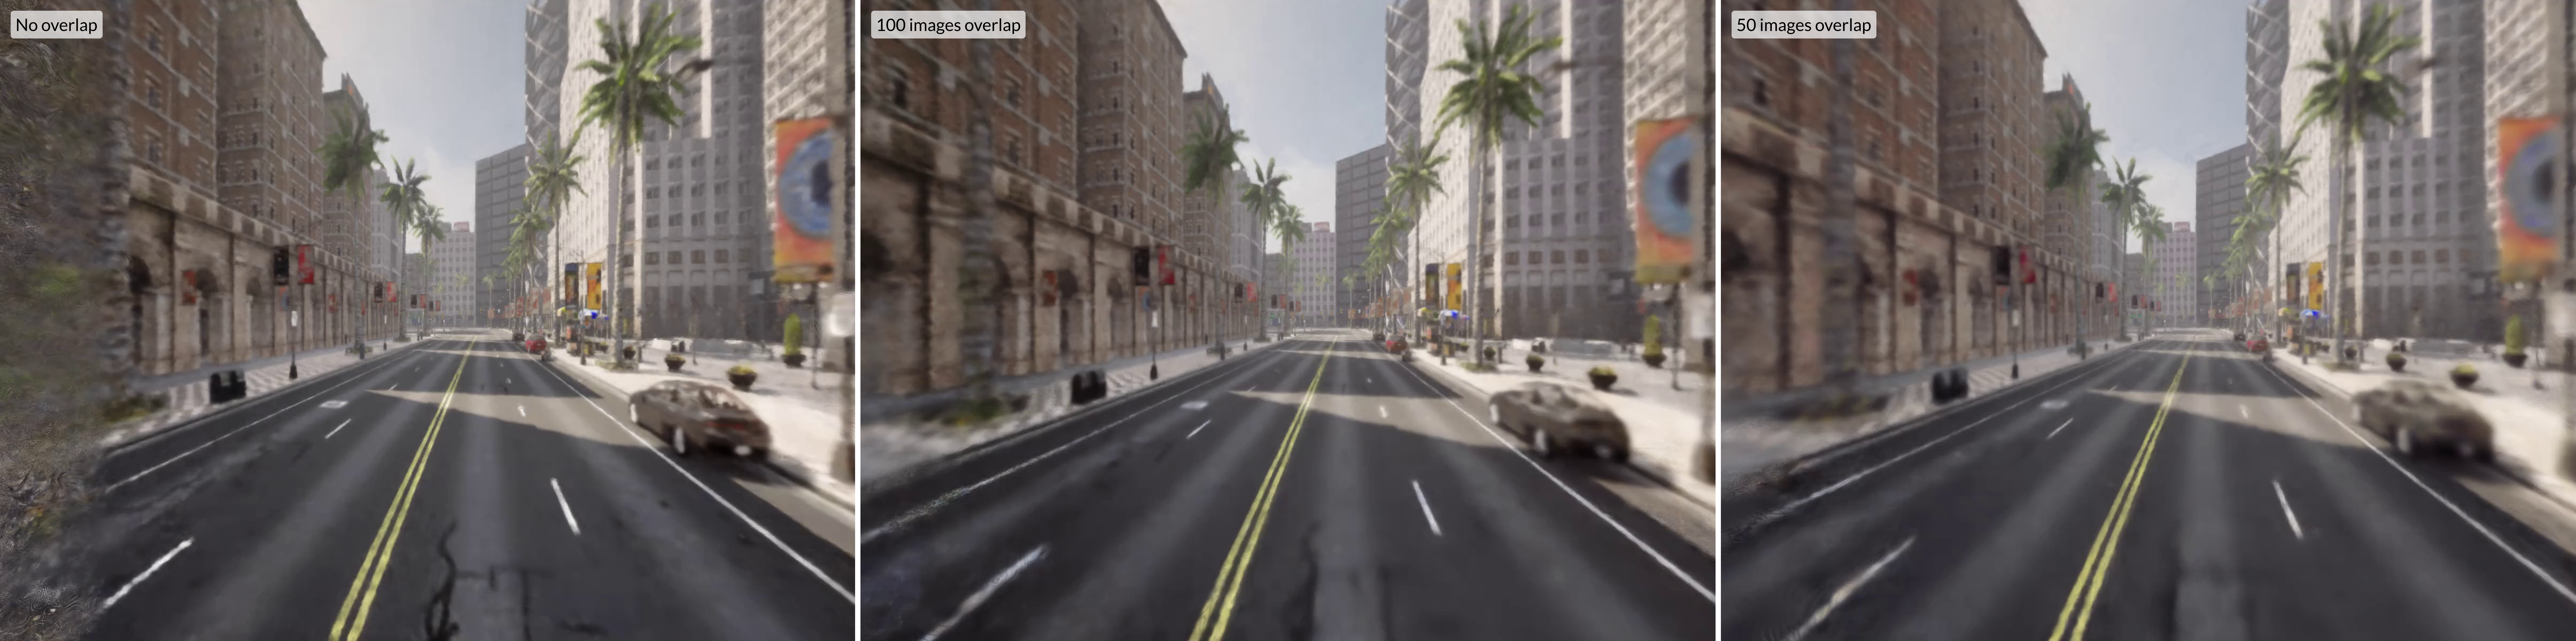
\includegraphics[width=1.0\textwidth]{figures/overlap.png}
    \caption{Comparison of Block-NeRF trained with 0, 50 and 100 images overlap, respectively.}
    \label{fig:overlap}
\end{figure}


As shown in \autoref{fig:overlap}, an increase in $\delta$ results in a significant reduction in the visible overlap between the blocks. Correspondingly, as indicated in \autoref{tab:block-nerf-overlap-comparison}, an increase in $\delta$ leads to a decline in NeRF quality across all three metrics. These findings suggest that it is necessary to identify a suitable value of $\delta$ that minimizes the visible overlap between blocks, while simultaneously maintaining high NeRF quality.
















\section{Experiment 5: Real Data}
The implementation of the real data-capture pipeline and the subsequent \texttt{NAPLabDataParser} allows the end-to-end pipeline to be run with data captured from the NAPLab car. With the ability to conduct experiments on real data, we want to investigate the quality of the capture, if the captured data is suitable for training NeRFs, how the camera poses estimated from the GPS compare to the camera poses approximated with COLMAP, how splitting up the data and leveraging a Block-NeRF approach affects performance, and how camera optimization affects the results.

In order to test the aforementioned aspects, eight different pipeline runs are conducted on the three datasets previously presented in \autoref{fig:naplab-dataset}. The experimental results for dataset 1 are presented in \autoref{tab:trip086-results}. As the results for datasets 2 and 3 show similar results, they have been moved to \autoref{app:real-data}.

\begin{table}[ht]
\centering
\setlength{\tabcolsep}{6pt}
\renewcommand{\arraystretch}{1.5}
\begin{tabular}{l | C{2.2} C{1.3} C{1.3} c}
\hline
\textbf{Description} & \textbf{PSNR $\uparrow$} & \textbf{SSIM $\uparrow$} & \textbf{LPIPS $\downarrow$} & \textbf{Time processing} \\
\hline
COLMAP w/ optimizer           & 21.990341 & 0.791958 & 0.404055         & 00:26:45 \\
COLMAP w/o optimizer          & 24.589824 & 0.862041 & 0.272113         & 00:26:45 \\
COLMAP w/ optimizer, 4 BNs    & 22.581596	& 0.79431075 & 0.25169325   & 00:26:45 \\
COLMAP w/o optimizer, 4 BNs   &\cellcolor{green} 27.264171 &\cellcolor{green} 0.8992085 &\cellcolor{green} 0.1979095       & 00:26:45 \\
GPS w/ optimizer              & 20.001791 & 0.753200 & 0.491038         & 00:00:00 \\
GPS w/o optimizer             &\cellcolor{red} 17.044231 & 0.737539 &\cellcolor{red} 0.550054         & 00:00:00 \\
GPS w/ optimizer, 4 BNs       & 20.115084 & 0.74115775 & 0.39719275     & 00:00:00 \\
GPS w/o optimizer, 4 BNs      & 19.37362825 &\cellcolor{red} 0.73673875 & 0.5112605    & 00:00:00 \\
\hline
\end{tabular}
\caption[Results from experiment 5: Real data]{Results from training NeRF on dataset 1. The transformation matrices are approximated with COLMAP or estimated from GPS-readings. "BN" is an abbreviation of Block-NeRF and the resulting metric score is averaged across the 4 NeRFs evaluations.}
\label{tab:trip086-results}
\end{table}



\begin{figure}[h]
    \centering
    \includegraphics[width=1.0\textwidth]{figures/trip086-comparison.png}
    \caption{Comparison of the different methods used to train the NeRF on dataset 1.}
    \label{fig:trip086-comparison}
\end{figure}



The results highlight interesting trade-offs between the applied approaches. Notably, the Block-NeRF runs with camera poses approximated by COLMAP without further optimization, yielded the best metrics across all the experiments. Disregarding both Block-NeRF runs, the NeRF trained on images with camera poses approximated with COLMAP and not further optimized yielded the best quantitative results. In contrast, the experiments leveraging GPS readings for camera pose approximations with or without optimization were less successful across all metrics, with the non-optimized GPS approach scoring the lowest across all three metrics.


% Of the runs that don't leverage the naive Block-NeRF approach, the run with camera poses approximated with COLMAP and further optimized camera poses achieves the significantly best PSNR. The COLMAP run without optimizer achieves best SSIM and LPIPS, although the metrics are very similar to the run with optimizer. The qualitative results from the two runs are very different. The run with optimized camera poses appear much more blurry than the one without optimized camera poses.


\begin{comment}
- As expected, the camera optimizer provides better results than the contrary on real data with imperfect camera poses. Atleast it ha a significantly higher PSNR, how do they compare qualitatively?
- As with the synthetic data, the optimized runs appear more blurry, but still achieves better scores on the metrics.


In the set of experiments that did not implement the naive Block-NeRF approach, the results display noteworthy distinctions between different methodologies. The experiment wherein camera poses were approximated using COLMAP and subsequently optimized rendered the highest Peak Signal-to-Noise Ratio (PSNR). This particular experiment demonstrates superior performance in preserving original image detail and quality.

However, interestingly, the experiment utilizing COLMAP without any subsequent optimization yielded the best results in terms of the Structural Similarity Index Measure (SSIM) and the Learned Perceptual Image Patch Similarity (LPIPS). Despite these metrics being extremely close to the COLMAP run with optimization, their distinction in results is worth noting.

Delving deeper into qualitative outcomes, a stark contrast is observed between the two COLMAP runs. The experiment leveraging optimized camera poses generated results with a distinctly higher degree of blurriness compared to its counterpart that did not utilize optimized poses.

This observation highlights the intriguing impact of pose optimization on image clarity and indicates that while certain metrics might be optimized, subjective visual quality and the overall objective might vary significantly. These results collectively underline the complex interplay between technical metrics and perceptual outcomes in the realm of NeRF generation.
\end{comment}


\section{Experiment 6: Novel Views Along Altered Trajectory} \label{sec:altered-trajectories}

An important application of NeRFs is their ability to synthesize high-quality images from novel viewpoints. Although there are many applications for this, one of those is training and evaluating self-driving vehicles. In this section, we will investigate how a NeRF trained on self-captured synthetic and real data can be used to create camera paths and render novel views not previously observed in the dataset. \autoref{fig:altered-trajectories} shows four different camera paths created in Nerfstudio for trained NeRFs.

% In order to investigate how our self-captured data performs for this purpose 
% As previously discussed, NeRF is employed in autonomous vehicle pipelines for this exact purpose.
%This capability could prove particularly useful in applications 
% you need to expand a dataset, e.g. in a machine learning setting, much like you would employ data augmentation.
% One important application of NeRFs is their ability to synthesize images from previously unseen viewpoints, not present in the original dataset. 
% This capability could prove particularly useful in applications where you need to expand a dataset, e.g. in a machine learning setting, much like you would employ data augmentation.


%\begin{figure}[h]
    \centering
    \includegraphics[width=1.0\textwidth]{figures/unseen-trajectories-v2.png}
    \caption{Previously unseen trajectories being rendered by defining a new camera path for the trained NeRF.}
    \label{fig:unseen-trajectories-v2}
\end{figure}
%\begin{figure}[h]
    \centering
    \includegraphics[width=1.0\textwidth]{figures/unseen-trajectories-real-data.png}
    \caption{Previously unseen trajectories being rendered by defining a new camera path for the trained NeRF. Left) From dataset 3 with a trajectory into a road sign, right) from dataset 1 with a swerving trajectory across the curb.}
    \label{fig:unseen-trajectories-real-data}
\end{figure}
\begin{figure}[h]
    \centering
    \includegraphics[width=1.0\textwidth]{figures/altered-trajectories.png}
    \caption[Results from experiment 6: Altered trajectories]{Previously unseen trajectories being rendered by defining a new camera path for the trained NeRF. Image 1 illustrates a trajectory deviating across a traffic light zone, while image 2 shows a trajectory veering into the opposing lane. Image 3, derived from dataset 3, portrays a trajectory directed towards a road sign, and Image 4, derived from dataset 1, presents a trajectory swerving over the curb.}
    \label{fig:altered-trajectories}
\end{figure}




% For discussion
% The scene has only been seen from a very limited number of views. In order to generate high-quality novel views, the same scene should be observed from multiple viewpoints.
\chapter{Discussion}
This chapter discusses and analyzes the results of our experiments, highlighting their significance in the context of the research questions. We also reflect on any limitations of the thesis and attempt to address the research questions based on the findings.

\section{Defining a baseline}

\begin{comment}
Points to discuss:
- Main point: Discuss the process of choosing which experiments was chosen.
- There might have been other experiments that should've been included in deciding the baseline.
- The way to choose which experiment goes forward could've been done differently.
- Although one experiment seem to do better with the current chosen setup, it might've done worse in another setup.
\end{comment}

In order to define a baseline for capturing data for training NeRFs, I chose five experiments to test: camera setup, capacity, number of frames, image size, and vehicle speed. These experiments were chosen based on heuristics and knowledge of what contributes to good NeRF results, such as well-lit scenes and non-blurry images. While the chosen experiments consider important factors for capturing data for NeRFs, there may have been other experiments that could have been included in defining the baseline. It's also important to weigh the fact that the best-performing settings in one experiment may not generalize to other setups. Overall, the process of defining a baseline is an iterative one that requires careful consideration of various factors and a willingness to continuously improve and refine the baseline.

\subsection{Camera setup}

The camera setup used in the experiment was arbitrary and may not reflect how cameras are typically rigged on cars. Future research could explore more realistic camera setups to improve the generalizability of the results. Additionally, the camera setups used in the study were sparse, with only a few cameras at specific angles. It is possible that other camera setups could yield even better results.

The results of the experiment showed relatively little difference in the quantitative metrics across the camera setups tested. However, camera setup 1 with two cameras at -10$^{\circ}$ and 10$^{\circ}$ yaw produced the highest SSIM and lowest LPIPS scores, indicating that it produced the most visually similar and perceptually pleasing images. One possible explanation of this result can be the level of overlap between the captured images the given setup provides. Both cameras have a field of view of $90^\circ$ and are mounted in the same location, resulting in a $70^\circ$ overlap between the images in the training data. This overlap means that when the model trains on an image from one of the cameras, it necessarily also trains on approximately three-quarters of the scene captured from the other camera. Because the evaluation set is a subset of the training images, it's fair to assume that the model should score high on the respective metrics.


\begin{comment}
- The position of the camera was arbitrary. Could've done more research into how cameras on cars usually are rigged.
- The camera setups are very sparse, a lot of different possibilities.

Results:
- Relatively little difference in the quantitative results.
- Why did the -10 and 10 yaw yield the best SSIM and LPIPS?
- The evaluation images are a subset of the training images. Because the -10 and 10 have a lot of overlap, they have a lot of common training data which will allow the model to learn the scene which it is evaluated on, in turn yielding high scores on the chosen metrics.


This overlap allows the model to train and learn the scene which it is evaluated on, because the evaluation set is a subset of the training images, more than the other setups, and it'll naturally score high on the respective images.

the model to train on the partial scene with two times the amount of data, and since the evaluation set is a subset of the training images, it'll naturally score high on the respective images.

\end{comment}










\subsection{Capacity}
% Summarize the important discussion added in the experiment
As stated in the experiment's section, the longest segment was selected for the baseline despite achieving the lowest scores across the metrics. This was done to ensure that the scene encompasses a diverse range of environments, including straight roads, curves, intersections, and varying lighting conditions.

% New discussion
In the qualitative analysis of the capacity results, it's evident that the quality of the renders degrades as the segment's length increase. The most prominent deterioration is the increase in blur. A reason why PSNR remains relatively constant across the different experiments is probably in part because PSNR has been shown not to capture blur well \cite{videoprocessingai}, as exemplified by \autoref{fig:psnr-critique}. This example demonstrates the importance of evaluating the different metrics, as both SSIM and LPIPS are good metrics for capturing blur.

% https://videoprocessing.ai/metrics/ways-of-cheating-on-popular-objective-metrics.html
\begin{figure}[ht]
    \centering
    \includegraphics[width=1.0\textwidth]{figures/psnr-critique.png}
    \caption{Comparison of an image depicting a boat that has been subjected to various types of distortions.}
    \label{fig:psnr-critique}
\end{figure}

















\subsection{Number of frames}

%- The captured images are very similar
%- The default dataset size in Nerfstudio is 300 images
%- Show a mathematical proof of why more images would make sense

To comprehend the outcomes of this experiment, it would be beneficial to look into how the number of frames and the image size impact the training process. We train for 15'000 iterations where each iteration uses 4096 pixels. This results in $\sim61$ million pixels being viewed throughout a single training. With 225 images and an image resolution of $600 \times 450$, we have $\sim61$ million pixels. That means that by the end of the training, approximately all of the input pixels were trained on. A dataset containing more than 225 images and corresponding camera poses would leave abundant pixels, and any fewer would lead to pixels being trained on multiple times. This calculation would entail that the results should be relatively similar for all experiments with 1231, 615, 411, 307, and 247 images respectively. But, there is a significant drop in PSNR from experiments 1 to 4. The drop in PSNR leads me to believe another important factor is the variety in the dataset.


% TODO: I should discuss other options as to why the number of frames affect the metrics in the way it does.












\subsection{Image size}
Based on the metric scores, it might seem counterintuitive that the lowest resolution of $200 \times 150$ performed best. However, a deeper look at the qualitative results in \autoref{fig:image-size-comparison} reveals a different narrative. Despite lower resolutions yielding higher scores on metrics, they seem to fail in capturing fine-grained details, resulting in less visually pleasing images. On the other hand, higher-resolution images allow the NeRF model to capture and replicate more intricate details, leading to superior visual outcomes, albeit with lower metric scores. This difference can be attributed to the higher sensitivity of metrics to minor discrepancies and noise in high-resolution images, potentially causing significant metric score reductions despite only minimal perceptual differences.

Given these considerations, the chosen resolution of $400 \times 300$ for the following experiments is a balanced choice, considering both the metrics and the perceptual image quality. Furthermore, it aligns well with the chosen number of frames from the previous experiment, as the combined configuration will allow training to cover about 84\% of the input pixels.

\begin{comment}
The qualitative assessment shows clear evidence of higher resolution images leading to higher fidelity renders, although the metrics suggest otherwise. When using lower-resolution images, the metrics may become less sensitive because they are less affected by small differences between the synthesized and ground-truth images. This is because lower-resolution images have fewer pixels, which can make the metrics less precise in measuring the perceptual similarity between the images. However, using lower-resolution images can also lead to a loss of detail and fidelity in the synthesized images. When comparing low-resolution images with high-resolution images, these metrics may become less effective because the high-resolution images are more sensitive to small differences between the synthesized and ground-truth images. In other words, the NeRF may generate high-quality images that are perceptually similar to the ground-truth images, but small differences in the pixel values or noise can cause a significant decrease in the metric scores.

The chosen resolution of $400 \times 300$ aligns well with the chosen number of frames from the previous experiment. With 2 ticks per image, $\sim615$ images for the baseline, we have $\sim73$ million pixels. The training will cover about 84\% of the input pixels.

This might be a special case for synthetic data where we have perfect camera poses. With higher-resolution images, the requirement for accurate camera poses increases as the camera poses have to be aligned pixel perfect with the image.
\end{comment}












\subsection{Vehicle speed}
The reason why the faster runs achieve worse results might be attributed to the motion blur and temporal artifacts that can occur when the vehicle is moving fast. In CARLA these effects are added as part of the post-processing of the captured camera image. At higher speeds, the motion of the vehicle can cause blurring and distortion in the captured images, which can reduce the quality of the data and make it more difficult for the NeRF to learn the underlying 3D scene structure and appearance. In contrast, slower vehicle speeds can reduce the amount of motion blur and temporal artifacts, resulting in clearer and more detailed images. Another side effect of driving slower is that it leads to an increased amount of images captured. At 50\% speed, the dataset consists of 1095 images, in contrast to the 429 images captured at 200\% speed.


% The reason for this can be attributed to the motion blur and temporal artifacts that can occur when the vehicle is moving too fast. At higher speeds, the motion of the vehicle can cause blurring and distortion in the captured images, which can reduce the quality of the data and make it more difficult for the NeRF to learn the underlying 3D scene structure and appearance. In contrast, slower vehicle speeds can reduce the amount of motion blur and temporal artifacts, resulting in clearer and more detailed images. Another side effect of driving slower is that it leads to increased amount of images captured. At 50\% speed, the dataset consists of 351 images, in contrast to the 131 images captured at 200\% speed.
























\subsection{Combined baseline}
% I might not need the initial "Defining a baseline" if I sum it up in this chapter.
\begin{description}[leftmargin=!,labelwidth=\widthof{RQ 1:}]
\item[\textbf{RQ 1:}] What are the critical factors that need to be considered when capturing synthetic data for training NeRF models, and how do they impact the performance of the resulting models?
\end{description}


From the experiments discussed above, it's evident that they all contribute to the quality of the data capture, which in turn contributed to the quality of the image synthesis from the resulting NeRF. Nevertheless, it is challenging to quantify the extent to which each of the different configurations affects the quality of the final baseline results.

Looking at the experiments separately, image resolution had the largest span between the quantitatively best and worst metrics. Nevertheless, the qualitative results indicated that the quantitative comparison didn't convey a fair comparison of the render-quality. Due to this, the capacity-experiment could be the experiment with the most impact on the final result.

In conclusion, when capturing synthetic data for training NeRF models, it's important to consider the camera setup, segment length or scene size, dataset size, image size, and vehicle speed. Each of these parameters presents unique influences on the quality of the data captured, and in turn, the performance of the resulting NeRF models.


\begin{comment}
The critical factors that must be considered when capturing synthetic data for training NeRF models, as inferred from the discussed baseline experiments, encompass camera setup, capacity, number of frames, image size, and vehicle speed. Each of these factors demonstrates a unique impact on the performance of the resulting models.

Camera setup plays a significant role in determining the quality of data captured for NeRF models. The experiments revealed that certain camera arrangements, specifically a setup with two cameras at -10$^{\circ}$ and 10$^{\circ}$ yaw, can result in superior SSIM and LPIPS scores, indicating more visually similar and perceptually pleasing images. This finding can be attributed to the degree of overlap between images captured by each camera in the setup. However, the experiments also highlight that camera arrangements were arbitrary and future research may investigate more realistic setups to better generalize the results.

The capacity, or the length of the road segment covered, also impacts the performance of the NeRF models. Even though longer segments led to lower scores across the metrics, these were still selected as the baseline to ensure a diverse range of environmental exposure for the model. It was noticed that the quality of renders deteriorated, especially in terms of increased blur, as segment length increased. Hence, the capacity of data has implications on the clarity and diversity of the training set, which could potentially influence the robustness of the model to diverse scenarios.

The number of frames in the dataset is another crucial factor. An optimal balance between the number of images and the image resolution is important for efficient training. In the experiments, a dataset with 225 images, each with a resolution of $600 \times 450$, covered approximately all of the input pixels by the end of training. However, a dataset with too many or too few images could result in either underutilization or overutilization of the pixels during training. Additionally, a decrease in PSNR with a drop in the number of frames points to the role of variety in the dataset.

The size of the images, or their resolution, has a complex impact on model performance. While higher resolution images contribute to higher fidelity renders, the metrics could suggest otherwise due to their increased sensitivity to minor differences in synthesized and ground-truth images. Hence, resolution can impact the quality of synthesized images and their metric scores, and it is crucial to align it with the number of frames for efficient coverage of input pixels.

Vehicle speed is a significant factor when capturing synthetic data, particularly due to the influence of motion blur and temporal artifacts on image quality. Faster vehicle speeds can lead to increased blur and distortion, making it challenging for the NeRF to learn the scene structure and appearance. Conversely, slower speeds provide clearer and more detailed images, improving the quality of the training data. Furthermore, slower speeds result in a larger dataset due to the increased number of images captured.

In conclusion, each of these factors—camera setup, capacity, number of frames, image size, and vehicle speed—has a unique and important influence on the quality of synthetic data captured for training NeRF models. Their careful consideration is essential for optimizing the performance of the resulting models.
\end{comment}








\section{Adding noise}
\begin{description}[leftmargin=!,labelwidth=\widthof{RQ 1:}]
\item[\textbf{RQ 2:}] How does the accuracy of initial camera poses and segment size influence the effectiveness of camera pose optimization, and is it possible to achieve equivalent results by optimizing rough camera poses directly, as opposed to pre-processing an approximation of accurate camera poses with tools such as COLMAP?
\end{description}

This research question addresses the effects of imperfect camera poses, frequently encountered in real-world scenarios due to GPS/GNSS inaccuracies, on the performance of camera pose optimization. We examine this by adding Gaussian noise to camera poses obtained from the CARLA pipeline, simulating real-world errors in the accuracy of these poses.

Despite Gaussian noise not perfectly replicating real-world noise distributions, its application allows a meaningful examination of camera pose optimization within our Nerfacto-pipeline. It is noteworthy that while the quantitative distinction between the non-optimized and optimized camera pose results might appear marginal, the qualitative contrasts outlined in both \autoref{fig:noise-short-segments} and \autoref{fig:noise-baseline-segments} deliver strong evidence of the camera pose optimization's effectiveness.

Particularly, the qualitative comparison highlights that the optimized camera poses generate consistently higher quality renders, even under significant noise levels. This is more discernible within shorter segments, where the optimization seems more efficient than in larger baseline scenes. This finding may be attributed to the previously discussed limitations in capacity, given that the camera optimization treats camera pose parameters as jointly optimized learnable parameters along with the RGB values.

Interestingly, the only instance where non-optimized poses yield superior results is when no noise is introduced. In such cases, the resulting render from non-optimized camera poses appears considerably sharper than its optimized counterpart, which may appear somewhat blurred. However, this outcome is most likely unique to synthetic datasets with perfect camera poses.


When examining the effectiveness of COLMAP pre-processing against the joint optimization of initial camera poses along with the other learnable parameters, it becomes evident that COLMAP tends to deliver superior performance. This observation holds particularly when the initial rough camera poses are influenced by a rather minor noise adhering to a Gaussian distribution with a standard deviation of $0.1^2$. Under these conditions, all three key metrics (PSNR, SSIM, LPIPS) associated with the NeRF lag behind those achieved by COLMAP, as can be seen from \autoref{tab:colmap-vs-poses} and \autoref{tab:exp-gaussian-noise}. Furthermore, when the noise's standard deviation is escalated to $0.5^2$, which is fair to assume could occur during real-world data capture, the metrics degrade even more significant compared to what COLMAP can deliver. While the processing time required by COLMAP might seem prohibitively lengthy for large datasets, this concern can be addressed by splitting the data into smaller sections. Thus, despite the initial time investment, COLMAP's superior performance merits consideration, particularly in scenarios with significant noise in initial camera poses.

\begin{comment}
The horizontal and vertical vectors in each experiment are subject to equal Gaussian noise. This approach may not fully capture the variability in noise that arises from realistic data capture scenarios, where factors such as the direction and speed of the vehicle can affect noise distribution. Nevertheless, the use of Gaussian noise enables the evaluation of the impact of camera optimization in the Nerfacto-pipeline.

While the difference in quantitative results between the runs with- and without camera pose optimization appear small, the qualitative comparison depicted in both \autoref{fig:noise-short-segments} and \autoref{fig:noise-baseline-segments} provides compelling evidence of its efficacy. Contrary to the NeRF that doesn't optimize the camera poses, the renders from the NeRF that optimized the camera poses remain relatively high-quality even when there is a substantial amount of noise added. This is particularly noticeable on shorter segments, where the optimization appears to perform even better than on the larger baseline scene. The observation can likely be ascribed to the capacity limitations previously discussed. This is because the camera optimization approach treats the camera pose parameters as learnable parameters that are jointly optimized with the RGB values.

The only scenario where NeRF with non-optimized camera poses outperforms its optimized counterpart is when no noise is added. In such cases, the resulting render is notably sharper than that produced by the optimized NeRF, which can appear more blurred. This finding is likely exclusive to synthetic datasets with perfect camera poses.
\end{comment}


\begin{comment}
DON'T NEED THIS SECTION BECAUSE THE COLMAP-RESULTS ARE DISCUSSED IN COMBINATION WITH THE NOISE-EXPERIMENT ABOVE.

\section{COLMAP vs. Absolute poses}
From the quantitative results, it appears COLMAP optimizes the camera poses similar to the camera pose optimization step in the Nerfacto-pipeline. When we turn off the camera pose optimization step, the perfect poses from CARLA enable even higher scores across the metrics and sharper renders.
\end{comment}





\section{Different models}
\begin{description}[leftmargin=!,labelwidth=\widthof{RQ 1:}]
\item[\textbf{RQ 3:}] How do different NeRF methods (NeRF, mip-NeRF, instant-ngp, Nerfacto) perform on unbounded scenes in terms of reconstruction quality and computational efficiency?
\end{description}


TODO



\section{Block NeRF}
\begin{description}[leftmargin=!,labelwidth=\widthof{RQ 1:}]
\item[\textbf{RQ 4:}] What are the technical challenges and considerations for implementing a functional approach for large-scale NeRF within the Nerfstudio API, and how does it compare to approaches not optimized for large-scale in terms of scalability, efficiency, and rendering quality?
\end{description}

Although the initial Block NeRF implementation is naive, both the quantitative and qualitative results provided demonstrate its efficacy. The renders of the shorter segments are much sharper and provide an overall better result. Although the results are very good, it's worth noting that the implementation requires substantially more computing. 





\subsection{Improving Block NeRF}
%The overlap between the blocks become substantially less visible with higher overlap values, $\delta$. When we increase $\delta$, we increase the dataset of each block leading to the capacity issue previously explored. In a production setting, it'll be important to tune all these parameters to effectively maximize quality across all blocks.

Although we solve the issue related to overlap, we see from \autoref{fig:block-nerf-frame-comparison} that the last frame in a block provides noticeably lower quality renders than the first frame in the next block. This is to be expected if the second block's data has been captured near the respective motive seen from both blocks. This difference could probably be further mitigated by experimenting with image-merging techniques, e.g. by rendering the view from both blocks and merging them with inverse distance weighing.

%Further improvements that could be done:
%- The details of the scenery in the second frame is clearly better than the first, which is expected as block number 2 has been trained on close-up images of the scene. This difference could be mitigated by looking into image-merging techniques such as inverse distance weighing.





\section{Implementation of CARLA to Nerfstudio pipeline}
Discuss the implementation.











\section{Generation of imperfect datasets}
\textbf{Unsure where to put this section}

One important application of NeRFs is their ability to synthesize images from previously unseen viewpoints, not present in the original dataset. This capability could prove particularly useful in applications where you need to expand a dataset, e.g. in a machine learning setting, much like you would employ data augmentation.

Given this thesis' focus on data captured by a driving vehicle, an apparent application is the generation of previously unseen vehicle trajectories. By capturing images from multiple viewpoints along a particular vehicle trajectory and subsequently training a NeRF on this data, the NeRF would enable the synthesis of new images depicting a previously unseen vehicle trajectory. This can be useful for a variety of applications, such as training autonomous driving systems. In \autoref{fig:nerfstudio-trajectory} you can see an example of how data from such an unseen trajectory can be generated by creating a camera path.

\begin{figure}[!h]
    \centering
    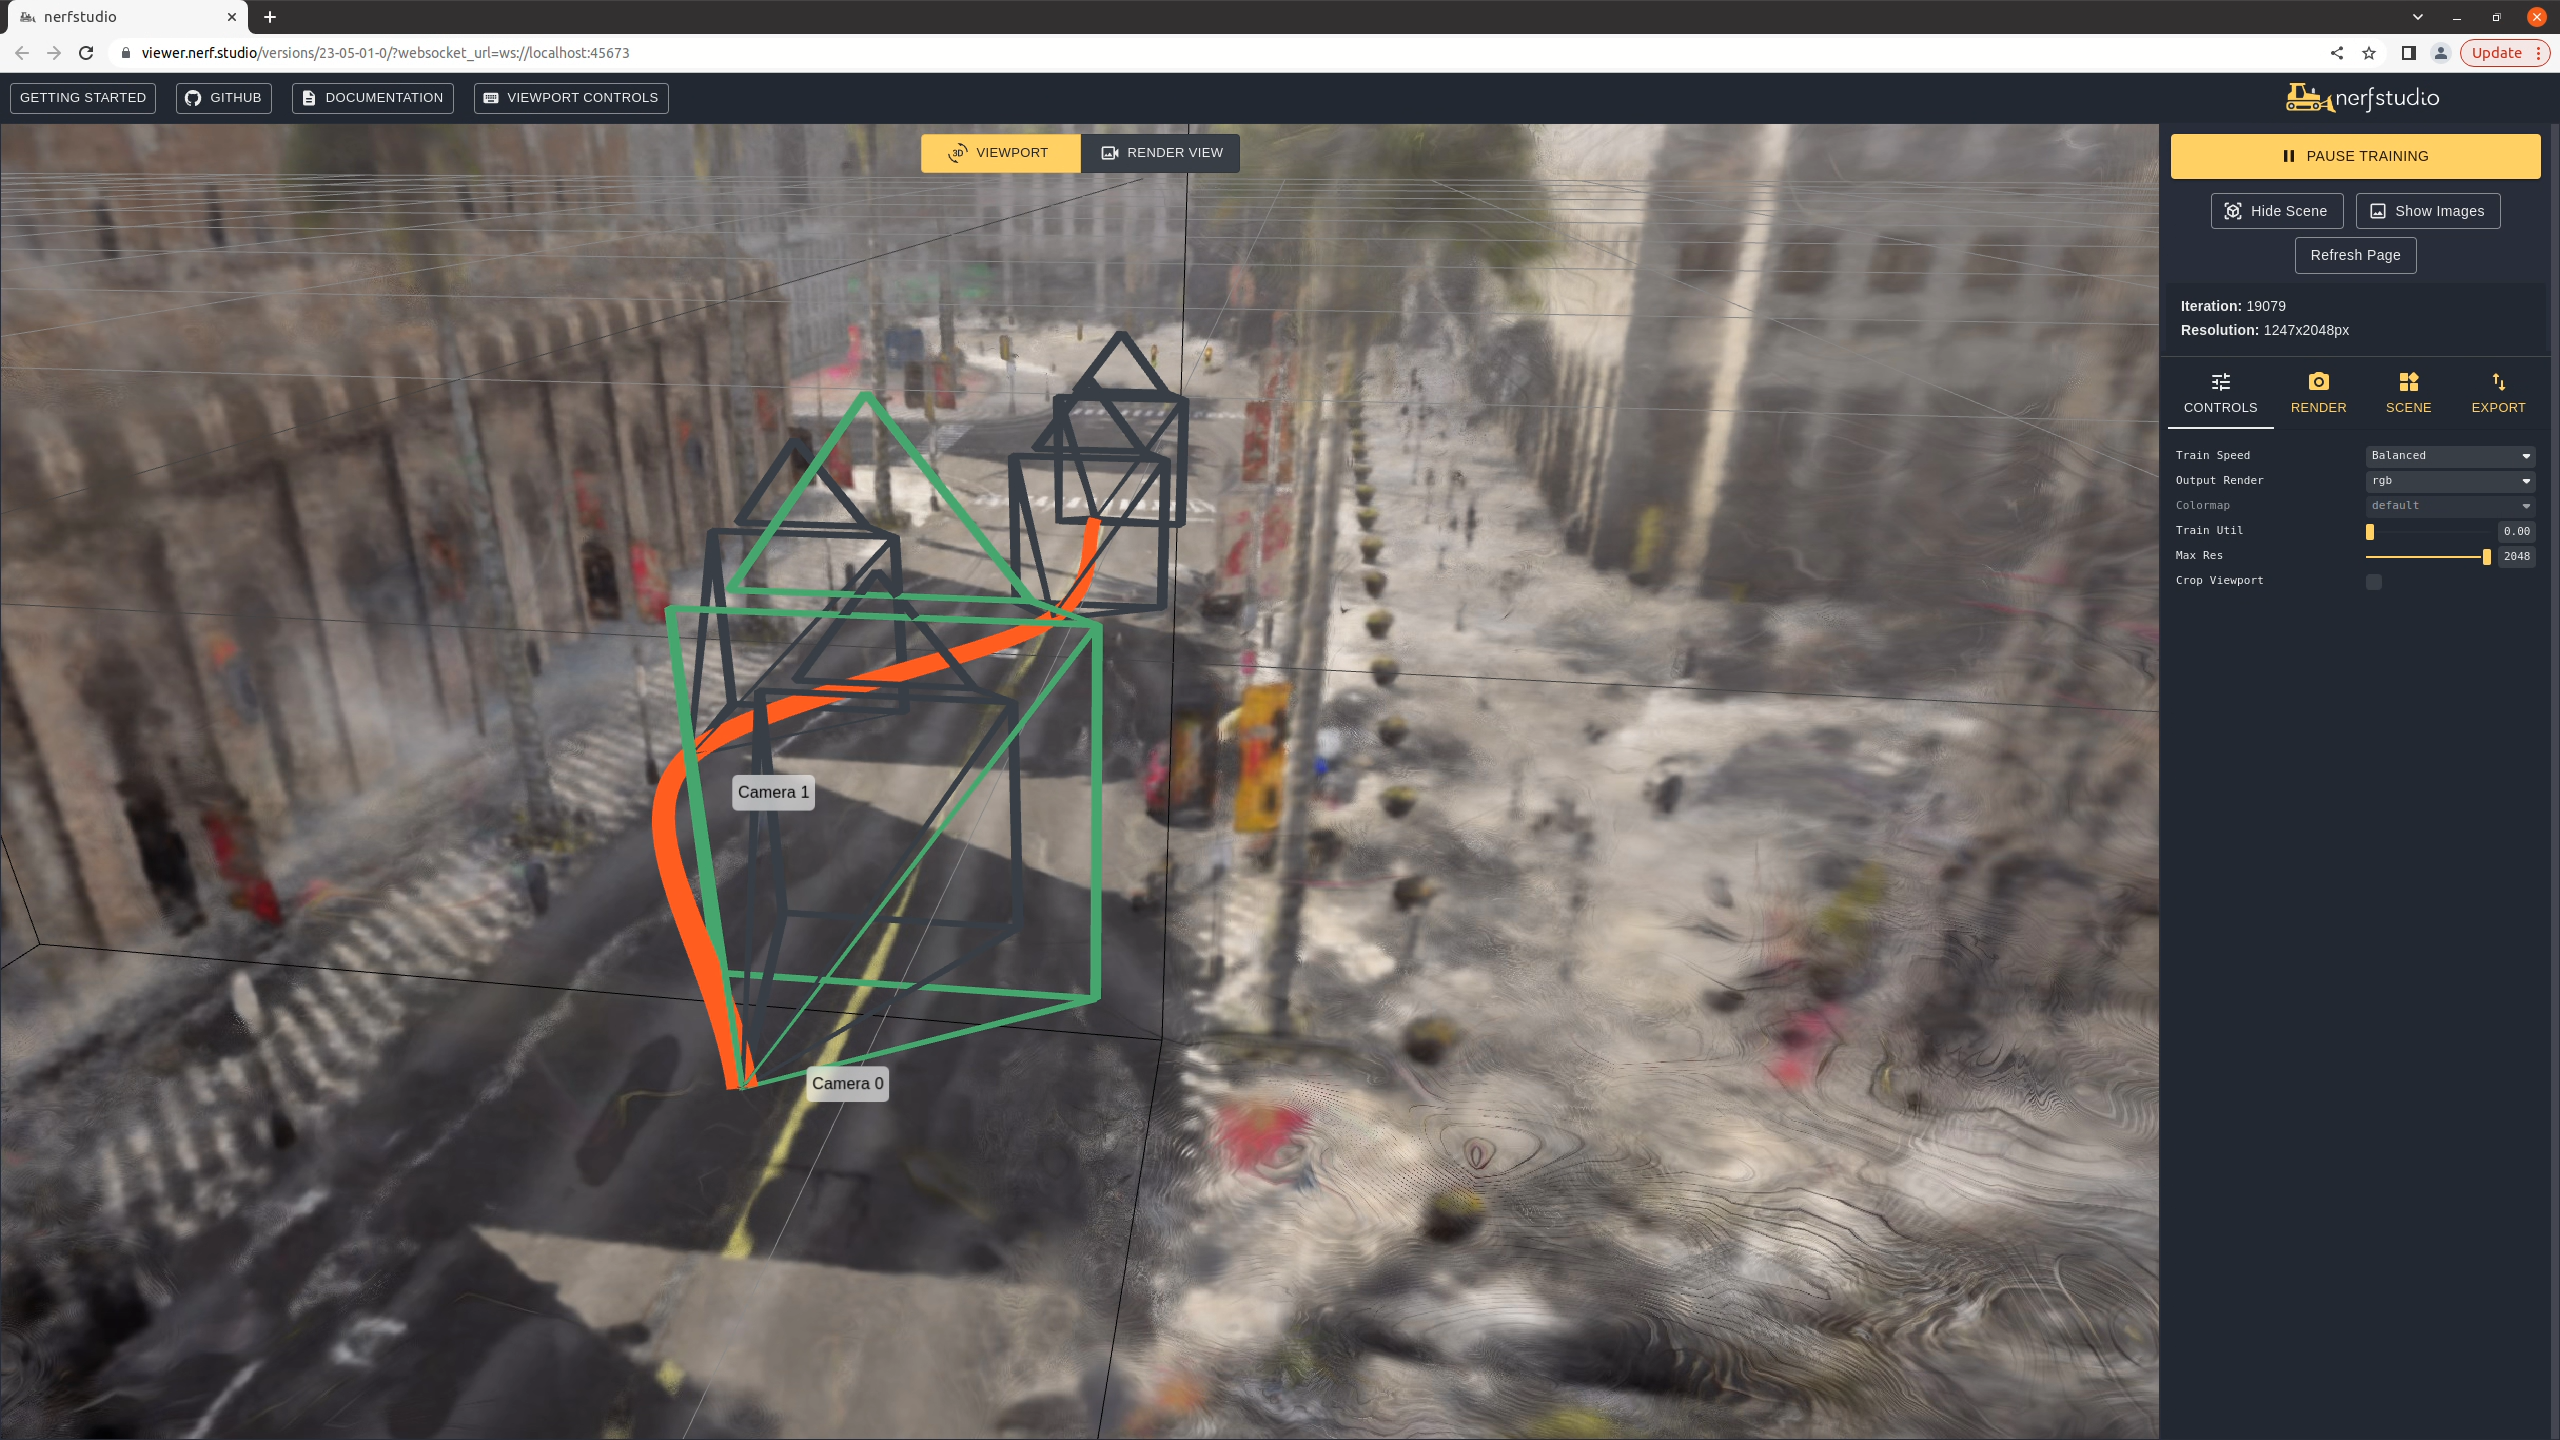
\includegraphics[width=1.0\textwidth]{figures/nerfstudio-trajectory.png}
    \caption{An arbitrary camera path trajectory created in Nerfstudio.}
    \label{fig:nerfstudio-trajectory}
\end{figure}














\section{Shortcomings}
\textbf{Just notes for now}
\subsection{Test the transferability from synthetic to real data}
There wasn't enough time to thoroughly test if the findings from the synthetic data would transfer to real data and contribute to better-performing NeRFs.
\chapter{Conclusion \& Future Work}

\section{Conclusion}
Conclude the thesis. Could create a holistic research goal that I could use to wrap up the thesis, or I could conclude what has been done, what worked and what should be looked into.



















\section{Future Work}
This section provides ideas related to NeRFs, synthetic data capture, and the extension to real-life data capture that were not covered in this report, but would be interesting to explore in future work.

\subsection{Improve pipeline for real-data capture}
Better estimate the rotation matrix from the collected data

\subsection{Large scale NeRF}
\begin{comment}
- Create a pipeline that enables the use of COLMAP for each segment in a more streamlined way. A succesful implementation should have significant implications on the quality of the resulting render.
- Mask transient objects using segmentation models
- Inverse distance weighing
- Visibility prediction
- Change backbone model to a model like F2 which have a different space warping algorithm, and should enable better results than using Nerfacto as the backbone model.
\end{comment}

\begin{itemize}
    \item Create a pipeline that enables the use of COLMAP for each segment in a more streamlined way. A successful implementation should have significant implications on the quality of the resulting render.
    \item Mask transient objects using segmentation models.
    \item Inverse distance weighing.
    \item Visibility prediction.
    \item Change backbone model to a model like F2 which has a different space warping algorithm, and should enable better results than using Nerfacto as the backbone model.
\end{itemize}

%\input{chapters/10-usage.tex}
%\input{chapters/10-structure.tex}




\chapter*{\bibname}
\printbibliography[heading=none]

%\input{chapters/papers.tex}

\appendix
\chapter{Additional Material} \label{app:additional}

\section{Parameters for the training in Nerfstudio} \label{sec:nerfstudio-train-parameters}

\subsection{Nerfacto}
\begin{table}[h]
    \begin{tabular}{|l|l|}
    \hline
    Description                                             & Default Value \\
    \hline
    How far along the ray to start sampling.                & 0.05 \\
    How far along the ray to stop sampling.                 & 1000.0 \\
    %Whether to randomize the background color.              & \"last\_sample\" \\
    %Number of samples per ray for the proposal network.     & \(256, 96\) \\
    Number of samples per ray for the nerf network.         & 48 \\
    Sample every n steps after the warmup                   & 5 \\
    Scales n from 1 to proposal\_update\_every over this many steps & 5000 \\
    Number of proposal network iterations.                  & 2 \\
    Use the same proposal network. Otherwise use different ones. & False \\
    Proposal loss multiplier.                               & 1.0 \\
    Distortion loss multiplier.                             & 0.002 \\
    Orientation loss multipier on computed noramls.         & 0.0001 \\
    Predicted normal loss multiplier.                       & 0.001 \\
    Whether to use proposal weight annealing.               & True \\
    Whether to use average appearance embedding or zeros for inference. & True \\
    Slope of the annealing function for the proposal weights & 10.0 \\
    Max num iterations for the annealing function.          & 1000 \\
    Whether use single jitter or not for the proposal networks. & True \\
    Whether to predict normals or not.                      & False \\
    \midrule\midrule
    Description of corresponding proposal density fields    & Default Value \\
    \hline
    Dimension of hidden layer           & 16 \\
    Hashmap size                        & $2^{17}$ \\
    Number of levels of the hashmap     & 5 \\
    Maximum resolution of the hashmap (density field 1)         & 64 \\
    Maximum resolution of the hashmap (density field 2)         & 256 \\
    \hline
    \end{tabular}
    \caption{An overview of the parameters in the default Nerfacto model}
    \label{tab:nerfacto-parameter-overview}
\end{table}

\subsection{Instant-ngp}
\begin{table}[h]
    %\centering
    \begin{tabular}{|l|l|}
    \hline
    \textbf{Description} & \textbf{Value} \\ 
    \hline
    Whether to create a scene collider to filter rays. & False \\
    Number of samples in field evaluation. & 24 \\
    Resolution of the grid used for the field. & 128 \\
    Contraction type. & Unbounded Sphere \\
    Cone angle & 0.004 \\
    Minimum step size for rendering. & 0.01 \\
    How far along ray to start sampling. & 0.05 \\
    How far along ray to stop sampling. & 1e3 \\
    Whether to use an appearance embedding. & False \\
    Whether to randomize the background color. & True \\ \hline
    \end{tabular}
    \caption{An overview of the parameters in the default Instant-ngp model}
    \label{tab:instant-ngp-parameter-overview}
\end{table}

\subsection{NeRF}
\begin{table}[h]
    %\centering
    \begin{tabular}{|l|l|}
    \hline
    \textbf{Description} & \textbf{Value} \\ 
    \hline
    Number of samples in coarse field evaluation & 64 \\
    Number of samples in fine field evaluation & 128 \\
    Specifies whether or not to include ray warping based on time. & False \\
    \hline
    \end{tabular}
    \caption{An overview of the parameters in the default NeRF model}
    \label{tab:nerf-parameter-overview}
\end{table}

\subsection{mip-NeRF}
\begin{table}[h]
    %\centering
    \begin{tabular}{|l|l|}
    \hline
    \textbf{Description} & \textbf{Value} \\ 
    \hline
    Whether to create a scene collider to filter rays.  & True \\
    Near plane collider-plane.                          & 2.0 \\
    Far plane collider-plane.                           & 6.0 \\
    The loss coeficcient for the coarse MLP.            & 1.0 \\
    The loss coeficcient for the fine MLP.              & 1.0 \\
    Number of rays per chunk during eval                & 4096 \\
    \hline
    \end{tabular}
    \caption{An overview of the parameters in the default mip-NeRF model}
    \label{tab:mip-nerf-parameter-overview}
\end{table}


\begin{comment}
    
Additional material that does not fit in the main thesis but may still be relevant to share, e.g., raw data from experiments and surveys, code listings, additional plots, pre-project reports, project agreements, contracts, logs etc., can be put in appendices. Simply issue the command \texttt{\textbackslash appendix} in the main \texttt{.tex} file, and make one chapter per appendix.

If the appendix is in the form of a ready-made PDF file, it should be supported by a small descriptive text, and included using the \texttt{pdfpages} package. To illustrate how it works, a standard project agreement (for the IE faculty at NTNU in Gjøvik) is attached here. You would probably want the included PDF file to begin on an odd (right hand) page, which is achieved by using the \texttt{\textbackslash cleardoublepage} command immediately before the \texttt{\textbackslash includepdf[]\{\}} command. Use the option \texttt{[pages=-]} to include all pages of the PDF document, or, e.g., \texttt{[pages=2-4]} to include only the given page range.

\cleardoublepage
\includepdf[pages=-]{appendices/NTNUProsjektavtale.pdf}
\end{comment}

\section{Results}

\subsection{Block NeRF}
% The full Block NeRF evaluation table. Only the condensed version containing the average across the different segments are included in the result-section

\begin{table}[ht]
\centering
\setlength{\tabcolsep}{6pt}
\renewcommand{\arraystretch}{1.5}
\begin{tabular}{l l | C{2.2} C{1.3} C{1.3}}
\hline
& \textbf{Description} & \textbf{PSNR $\uparrow$} & \textbf{SSIM $\uparrow$} & \textbf{LPIPS $\downarrow$} \\
\hline
0 & Segment 1 & 24.960262 & 0.815270 & 0.161623 \\
1 & Segment 2 & 25.660400 & 0.824085 & 0.164296 \\
2 & Segment 3 & 23.914209 & 0.755183 & 0.194245 \\
3 & Segment 4 & 23.363695 & 0.764547 & 0.216242 \\
\hline
\multicolumn{2}{l}{Average difference from one NeRF} &\cellcolor{green} 0.2768 &\cellcolor{green} 0.02277125 &  \cellcolor{red} -0.015 % Unsure if I'll include this
\end{tabular}
\caption{Results for each segment when the basline-segment spanning the entire block has been split into 4 Block-NeRFs.}
\label{tab:block-nerf-four-segments-full}
\end{table}


\begin{table}[ht]
\centering
\setlength{\tabcolsep}{6pt}
\renewcommand{\arraystretch}{1.5}
\begin{tabular}{l l | C{2.2} C{1.3} C{1.3}}
\hline
& \textbf{Description} & \textbf{PSNR $\uparrow$} & \textbf{SSIM $\uparrow$} & \textbf{LPIPS $\downarrow$} \\
\hline
0 & Segment 1 & 25.047100 & 0.826931 & 0.138852 \\
1 & Segment 2 & \cellcolor{green} 25.703838 & 0.831167 & 0.156331 \\
2 & Segment 3 & 24.924395 & 0.830144 & 0.149870 \\
3 & Segment 4 & \cellcolor{red} 22.726223 & \cellcolor{red} 0.713277 & \cellcolor{red} 0.207025 \\
4 & Segment 5 & 25.468483 & 0.837942 & \cellcolor{green} 0.131815 \\
5 & Segment 6 & 25.670006 & \cellcolor{green} 0.841962 & 0.147232 \\
6 & Segment 7 & 25.661350 & 0.820813 & 0.163685 \\
7 & Segment 8 & 25.070913 & 0.777114 & 0.154277 \\
8 & Segment 9 & 24.803871 & 0.814633 & 0.154028 \\
9 & Segment 10 & 23.693977 & 0.753770 & 0.185557 \\
10& Segment 11 & 23.936722 & 0.757462 & 0.179283 \\
11& Segment 12 & 24.584238 & 0.807874 & 0.144022 \\
\hline
\multicolumn{2}{l}{Average metrics of 12 block NeRF} & \cellcolor{green} 24.774259 & \cellcolor{green} 0.801090 & \cellcolor{green} 0.159331 \\
\multicolumn{2}{l}{Average metrics of 1 block NeRF} & \cellcolor{red} 22.515461 & \cellcolor{red} 0.654036 & \cellcolor{red} 0.424356 \\
\hline
\end{tabular}
\caption{Results for exp\_block\_nerf\_long\_path\_2-block\_10}
\label{tab:block-nerf-twelve-segments-full}
\end{table}

\end{document}
